% Sablon pentru realizarea lucrarii de licenta, conform cu recomandarile
% din ghidul de redactare:
% - https://fmi.unibuc.ro/finalizare-studii/
% - https://drive.google.com/file/d/1xj9kZZgTkcKMJkMLRuoYRgLQ1O8CX0mv/view

% Multumiri lui Gabriel Majeri, acest sablon a fost creat pe baza
% codului sursa a lucrarii sale de licenta. 
% Codul sursa: https://github.com/GabrielMajeri/bachelors-thesis
% Website: https://www.gabrielmajeri.ro/
%
% Aceast sablon este licentiat sub Creative Commons Attribution 4.0 International License.

\documentclass[12pt, a4paper]{report}

% Suport pentru diacritice și alte simboluri
\usepackage{fontspec}

% Suport pentru mai multe limbi
\usepackage{polyglossia}

% Setează limba textului la română
\setdefaultlanguage{romanian}
% Am nevoie de engleză pentru rezumat
\setotherlanguages{english}

% Indentează și primul paragraf al fiecărei noi secțiuni
\SetLanguageKeys{romanian}{indentfirst=true}

% Suport pentru diferite stiluri de ghilimele
\usepackage{csquotes}

\DeclareQuoteStyle{romanian}
  {\quotedblbase}
  {\textquotedblright}
  {\guillemotleft}
  {\guillemotright}

% Utilizează biblatex pentru referințe bibliografice
\usepackage[
    maxbibnames=50,
    sorting=nty
]{biblatex}

\addbibresource{bibliography.bib}

% Setează spațiere inter-linie la 1.5
\usepackage{setspace}
\onehalfspacing

% Modificarea geometriei paginii
\usepackage{geometry}

% Include funcțiile de grafică
\usepackage{graphicx}
% Încarcă imaginile din directorul `images`
\graphicspath{{./images/}}

% Listări de cod
\usepackage{listings}

% Linkuri interactive în PDF
\usepackage[
    colorlinks,
    linkcolor={black},
    menucolor={black},
    citecolor={black},
    urlcolor={blue}
]{hyperref}

% Simboluri matematice codificate Unicode
\usepackage[warnings-off={mathtools-colon,mathtools-overbracket}]{unicode-math}

% Comenzi matematice
\usepackage{amsmath}
\usepackage{mathtools}

% Formule matematice
\newcommand{\bigO}[1]{\symcal{O}\left(#1\right)}
\DeclarePairedDelimiter\abs{\lvert}{\rvert}

% Suport pentru rezumat în două limbi
% Bazat pe https://tex.stackexchange.com/a/70818
\newenvironment{abstractpage}
  {\cleardoublepage\vspace*{\fill}\thispagestyle{empty}}
  {\vfill\cleardoublepage}
\renewenvironment{abstract}[1]
  {\bigskip\selectlanguage{#1}%
   \begin{center}\bfseries\abstractname\end{center}}
  {\par\bigskip}

% Suport pentru anexe
\usepackage{appendix}

% Stiluri diferite de headere și footere
\usepackage{fancyhdr}

% Metadate
\title{Metode de clasificare pentru semnale EEG}
\author{Florete Fabian-Andrei}

% Generează variabilele cu @
\makeatletter

\begin{document}

% Front matter
\cleardoublepage
\let\ps@plain

% Pagina de titlu
\begin{titlepage}

% Redu marginile
\newgeometry{left=2cm,right=2cm,bottom=1cm}

\begin{figure}[!htb]
    \centering
    \begin{minipage}{0.2\textwidth}
        
\includegraphics[width=\linewidth]{logo-ub.png}
    \end{minipage}
    \begin{minipage}{0.5\textwidth}
        \large
        \vspace{0.2cm}
        \begin{center}
            \textbf{UNIVERSITATEA DIN BUCUREȘTI}
        \end{center}
        \vspace{0.3cm}
        \begin{center}
            \textbf{
                FACULTATEA DE \\
                MATEMATICĂ ȘI INFORMATICĂ
            }
        \end{center}
    \end{minipage}
    \begin{minipage}{0.2\textwidth}
        
\includegraphics[width=\linewidth]{logo-fmi.png}
    \end{minipage}
\end{figure}

\begin{center}
\textbf{SPECIALIZAREA INFORMATICĂ}
\end{center}

\vspace{1cm}

\begin{center}
\Large \textbf{Lucrare de licență}
\end{center}

\begin{center}
\huge \textbf{\MakeUppercase{\@title}}
\end{center}

\vspace{3cm}

\begin{center}
\large \textbf{Absolvent \\ \@author}
\end{center}

\vspace{0.25cm}

\begin{center}
\large \textbf{Coordonator științific \\ Conf. Dr. Sergiu Nisioi}
\end{center}

\vspace{2cm}

\begin{center}
\Large \textbf{București, Iunie 2025}
\end{center}
\end{titlepage}
\restoregeometry
\newgeometry{
    margin=2.5cm
}

\fancypagestyle{main}{
  \fancyhf{}
  \renewcommand\headrulewidth{0pt}
  \fancyhead[C]{}
  \fancyfoot[C]{\thepage}
}

\addtocounter{page}{1}

% Rezumatul
\begin{abstractpage}

\begin{abstract}{romanian}
Creierul uman constituie una dintre cele mai complexe și mai promițătoare arii de cercetare. Și, contrar faptului că a fost studiat intens de-a lungul timpului, încă nu avem un model destul de clar al modului în care acesta funcționează.

În această lucrare de licență am urmărit să explorez, să evaluez și să compar cât mai mulți algoritmi legați de interpretarea semnalelor emise de creier. Scopul principal este de a vedea gradul de interpretabilitate generat de diverși stimuli de scurtă durată. Lucrarea mea se diferențiază de restul lucrărilor din domeniul ERP prin tipul datelor folosite și prin specificitatea subiecților. Astfel, datele mele provin de la oameni specializați, și anume arhitecți ce au privit imagini specifice domeniului, mai exact coloane generate artificial.

Pe parcursul lucrării am implementat și comparat sistematic algoritmi documentați în literatura de specialitate.
\end{abstract}

\begin{abstract}{english}
The human brain represents one of the most complex and promising areas of research. And, although it has been intensely  studied throughout the years, we still do not have an accurate model of the way it functions.

In this thesis, I aimed to explore, evaluate and compare a wide range of algorithms related to the interpretation of brain-emitted signals. The main objective is to asses the degree of interpretability elicited by various short-duration stimuli. My work differs from the existing literature in the ERP domain via the type of data used and the specificity of the subjects. The data used comes from specialized subjects, more particularly architects that have been shown images specific to their domain, specifically, artificially generated columns.

Throughout the study, I systematically implemented and compared algorithms documented in the scientific literature.
\end{abstract}

\end{abstractpage}

\tableofcontents

% Main matter
\cleardoublepage
\pagestyle{main}
\let\ps@plain\ps@main

\chapter{Introducere}

\section{Context și motivație}
EEG-ul, sau Electroencefalograma, reprezintă o modalitate sigură și non-invazivă de a măsura activatea electromagnetică a creierului. Această măsurare este realizată printr-o cască ce conține mai mulți electrozi. Fiecare electrod în parte măsoara activiatea creierului in Volți. Aceste metode au aplicații intr-o multitudine de domenii. Cele mai folosite cazuri în literatura de specialitate sunt: detectarea fazelor somnului, a simptomelor epilepsiei, a sindromului Alzheimer, a diferitelor emoții puternice, precum tristețe, frică, fericire și, în domeniul de Brain-Computer interface, care se concentrează pe decodarea semnalelor creierului asociate cu mișcarea membrelor.
De-a lungul anilor, cercetătorii au obținut rezultate din ce în ce mai bune în domeniul clasificării emoțiilor induse de un stimul vizual. Dacă în anul 2016 cele mai bune modele se bazau pe SVM-uri și ajungeau la o acuratețe de 73\% \cite{ATKINSON201635} pentru clasificări între două clase, și 62\% pentru clasificări între trei clase, în anul 2020, modele precum TSception, ce se bazează pe rețele neuronale ating acurateți de peste 86\% \cite{TSception}. 

Totuși, în majoritatea cazurilor, stimulii induși sunt cauzați fie de evenimente de lungă durată: video-uri, ore întregi de somn, fie de evenimente binare, având clase target/non-target, de exemplu în cazul visual speller-elor \cite{visual_speller}. Mi-am propus să stabilesc dacă stimulii de scurtă durată au același potențial de a evoca răspunsuri capabile de a fi interpretate algoritmic precum cei de lungă durată în contextul unui grup de arhitecți care privesc coloane. Privirea unei coloane nu provoacă reacții emoționale puternice, dar tot are potențialul de a stârni anumite tipare de răspuns la nivelul creierului.

\section{Obiectivele Lucrării}
Scopul lucrării este de a prezice reacția subconștientă pe care o are mintea unui arhitect, provocată de afișarea pe durată scurtă a unor imagini reprezentând coloane generate artificial. În acest context, datele reprezintă semnale EEG de tip ERP (Event-Related Potential). În plus, prezicerea este făcută de-a lungul a trei dimensiuni afective: valență, excitare și dominanță. Abordarea are la bază presupunerea că ERP-urile reflectă reacții spontane, și faptul că, dacă un participant se gândește mai mult timp la o imagine începe să nu mai fie sigur dacă îi place sau nu. Spre îndeplinirea acestui scop, am folosit cât mai mulți algoritmi, comparându-i între ei pentru fiecare paradigmă de interpretare a semnalelor.

\section{Noțiuni preliminare despre paradigma ERP}

ERP (Event-Related Potential), sau, în traducere, potențial legat de eveniment, reprezintă răspunsul creierului uman asociat unui eveniment stimulant \cite{erp_introduction}. Evenimentele pot fi cauzate de diverși astfel de stimuli, de exemplu auditivi sau vizuali. Aceștia sunt captați prin intermediul unei căști EEG ce înregistrează activitatea creierului. ERP-urile pot fi mai departe împărțite în mai multe categorii în funcție de semnificația pe care dorim să o extragem din semnal. ERP-urile reprezintă în sine o fereastră de timp din semnalul original unde se află răspunsul subconștient al subiectului în fața stimulului prezentat. Înăuntrul acestor ferestre de timp pot apărea componente negative sau pozitive care variază semnificativ față de medie. Aceste componente sunt fie notate cu P (pentru vârfuri pozitive), sau cu N (pentru vârfuri negative). Datele pe care se bazează experimentele mele sunt legate de evenimente de tip P300, care, din denumire, reprezintă un vârf pozitiv ce apare după 300 milisecunde de la prezentarea stimulului.
\def\totalEpoci{5598}
\def\totalEpociTestare{0}
\def\totalEpociValentaPozitiva{1014}
\def\totalEpociValentaNegativa{942}
\def\totalEpociValentaNeutra{3642}
\def\crestereAcurateteAutoReject{10}
\def\nrParticipantiAntrenare{21}
\def\nrParticipantiValidare{2}
\def\nrParticipantiTestare{3}

\chapter{Metodologia}

\section{Setul de date}
\subsection{Preluarea datelor și formatul lor}
Datele constau în 26 de fișiere excel ce reprezintă citirile electrozilor subiecților experimentului.
Experimentul a constat într-un grup de arhitecți care au privit imagini generate cu inteligența artificială reprezentând coloane. Imaginile au fost prezentate timp de 0.4 secunde pe ecran, în încercarea de a captura o reacție subconștientă a participanților.
Ulterior, imaginile  privite sunt notate pe 3 criterii: V(Valence/Valență), A(Arousal/Excitare) și D(Dominance/Dominanță). 
Notele stimulilor sunt discretizate in 3 categorii: stimul negativ (note de la 1 la 3), stimul neutru (note de la 4 la 6) și stimul pozitiv (note de la 7-10). 
Scopul este astfel prezicerea categoriei de stimul provocat de o imagine. În pofida faptului că aceleași imagini au fost prezentate în mod repetat, în scopul evaluării pe cele trei dimensiuni, am considerat fiecare apariție ca fiind un eveniment independent, presupunând că răspunsul neuronal asociat fiecărei expuneri cât și punctajul acordat de participant poate varia. Motivul principal pentru care am ales această abordare a fost faptul că notele acordate nu au rămas constante de-a lungul przentării aceleiași imagini.

\begin{figure}[H]
    \centering
		\vspace{-1em}
    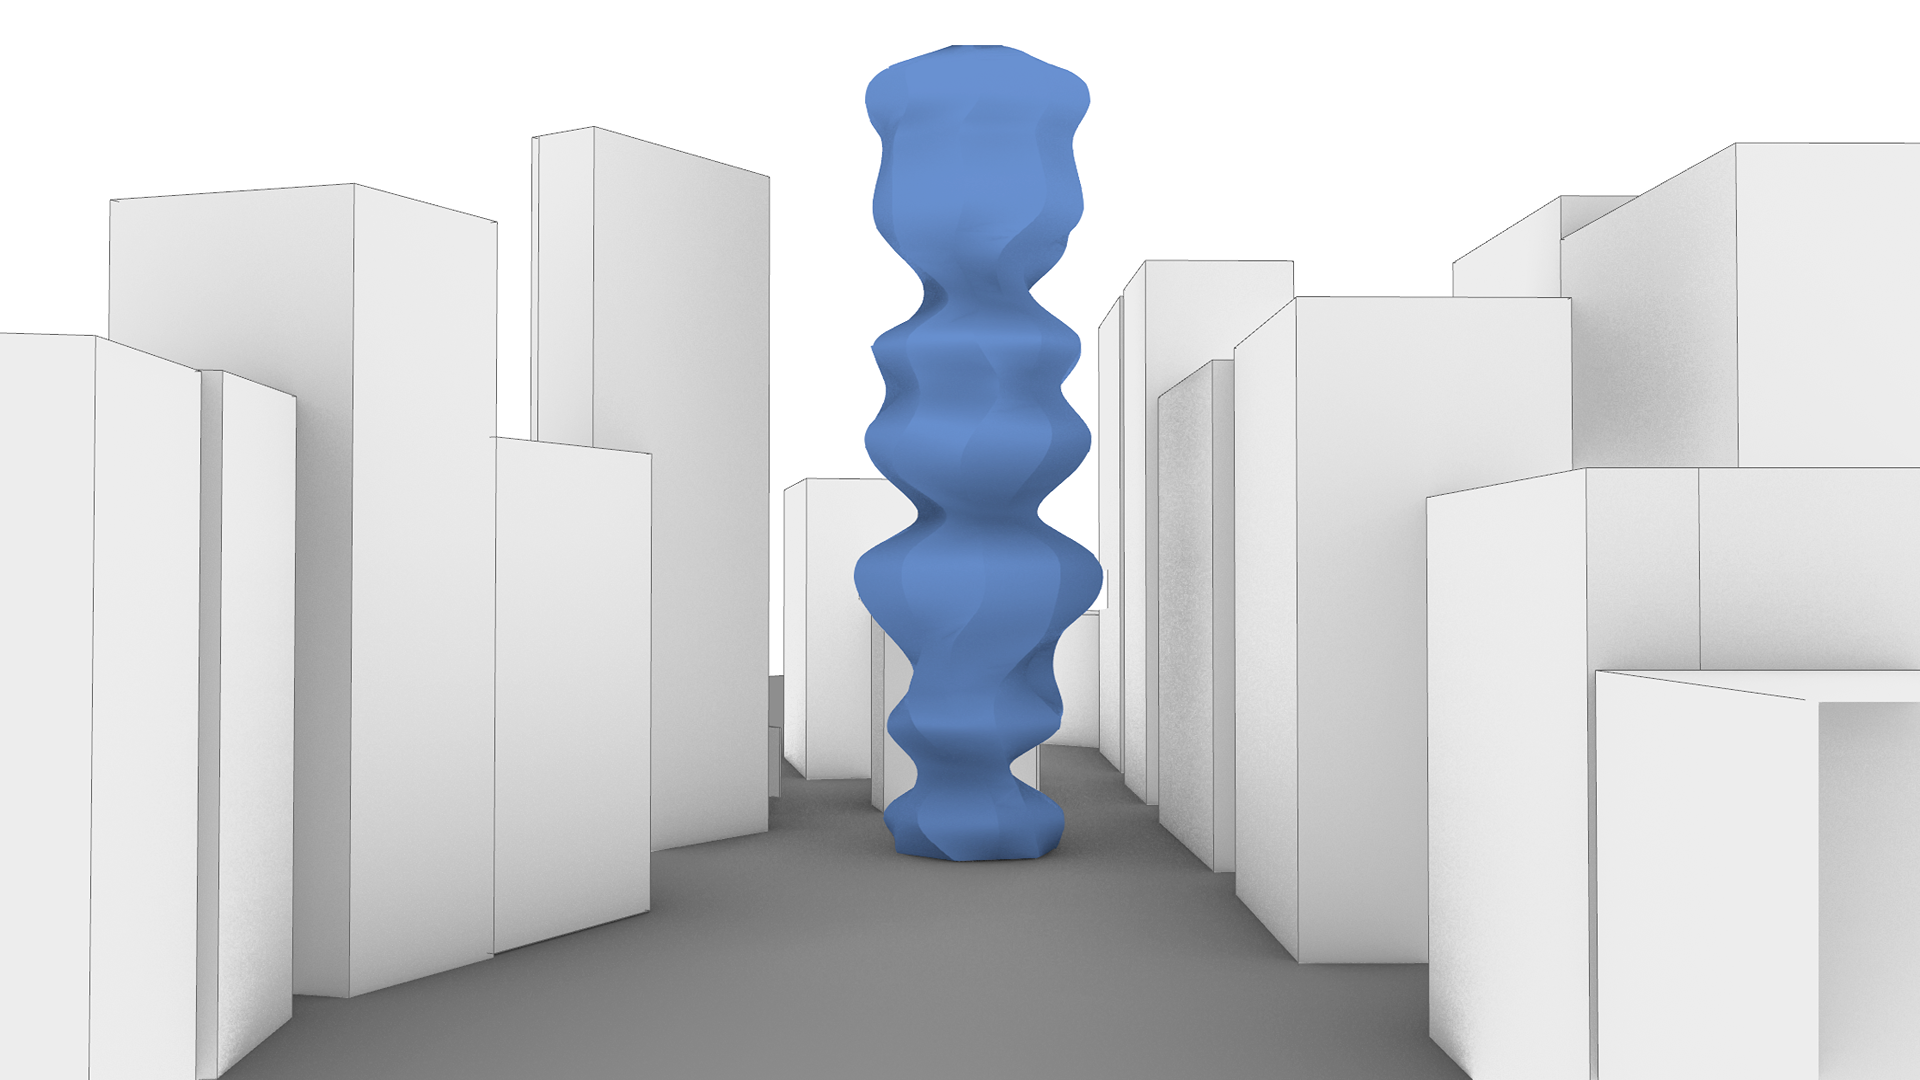
\includegraphics[width=0.5\linewidth]{stimul_image.png}
    \caption{Imagine generată artificial.}
		\vspace{-1em}
    \label{fig:enter-label}
\end{figure}

Fiecare fișier conține înregistrările corespunzătoare a 21 de electrozi plasați de-a lungul capului. 
Ei au măsurat activitatea creierului cu o frecvență de 300 Hz. 
Există și un canal de referință Pz care a fost folosit pentru a calibra măsurătorile. 
Astfel, el nu apare în setul de date. 
Corespunzător fiecărui sesiuni, am avut acces și la un fișier ce conține notele acordate de subiect fiecărei imagini văzute. 

\begin{figure}[H]
    \centering
		\vspace{-1em}
    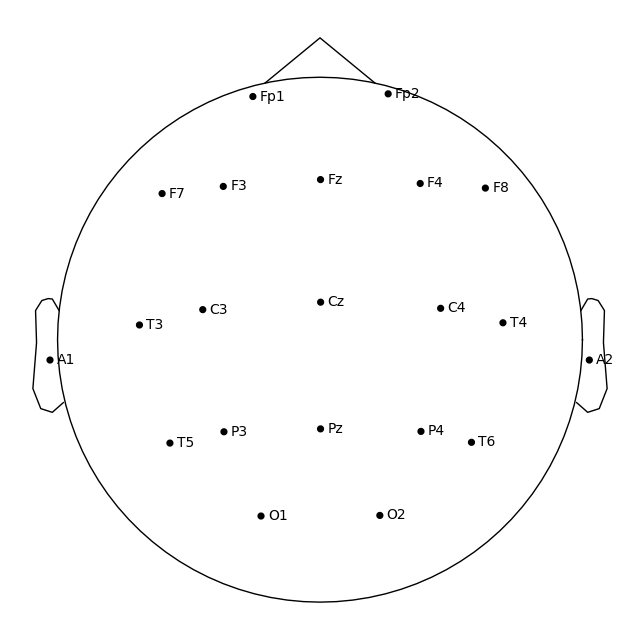
\includegraphics[width=8cm]{images/Sensor_positions_(eeg).png}
    \caption{Pozițiile electrozilor la nivelul capului.}
		\vspace{-1em}
    \label{fig:sensor_positions}
\end{figure}
Datele din formatul brut sunt încărcate folosind librăria Pandas \cite{reback2020pandas} din Python. Pe urmă, am mai adăugat coloane specifice etichetelor experimentului. Mai departe, am transformat datele în format .FIF și le-am încărcat în format de EEG-uri Raw din librăria MNE \cite{MNE}. Aceasta este specializată în încărcarea și preprocesarea datelor EEG.

\section{Preprocesarea datelor}
Înainte de a introduce datele în modele, acestea trebuiesc curățate. În primul rând, nu toate frecvențele sunt relevante pentru problemele de clasificare. Multe pot proveni din zgomot de fundal, mișcarea fizică a electrozilor sau interferențe electrice, precum zgomotul generat de rețeaua electrică sau imperfecțiunea electrozilor la capturarea semnalelor. Toata partea de preprocesare este parametrizată pentru a permite cautarea valorilor optime așa cum se poate vedea în figura \ref{fig:parametrizare} din Appendix.

% \setlength{\abovecaptionskip}{0pt}
% \setlength{\belowcaptionskip}{0pt}
% \begin{figure}
%     \centering
%     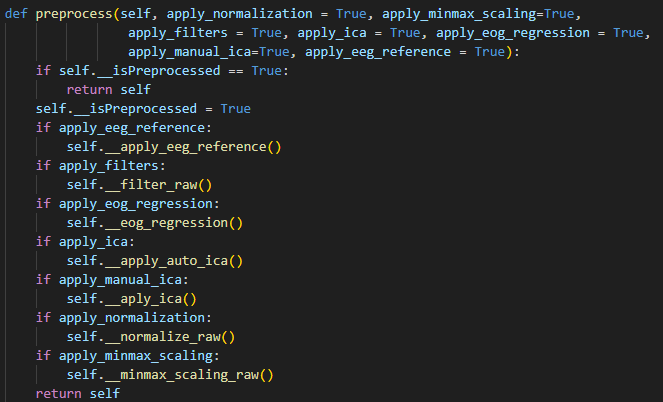
\includegraphics[width=10cm]{images/parametrizare.png}
%     \caption{Enter Caption}
%     \label{fig:enter-label}
% \end{figure}


\subsection{Filtrare, interpolare, ICA}

Literatura de specialitate sugerează să filtrăm datele astfel încât să păstrăm doar frecvențele între 4-40 Hz\cite{intro_to_mne}. Am folosit astfel un filtru trece-bandă care a păstrat doar frecvențele din acest interval. Cu ajutorul acestuia am eliminat frecvențele înalte cauzate de zgomotul electric al aparatului de măsurare, precum și drift-ul semnalului cauzat de modul în care aparatura a fost montată, neavând contact perfect cu scalpul.  %Modul de functionare al acestuia este următorul: este creeat un filtru în domeniul frecvențelor. Acest filtru este transpus în domeniul timp. Din semnalul original sunt luate bucăți segmentate. Ele sunt înmulțite cu o fereastră hamming pentru a elimina fenomenul de spectral leakage. Bucata segmentată este trecută prin operația de convoluție cu filtrul original și astfel este obținut un semnal filtrat.

\setlength{\abovecaptionskip}{0pt}
\setlength{\belowcaptionskip}{0pt}
\begin{figure}[H]
    \centering
		\vspace{-1em}
    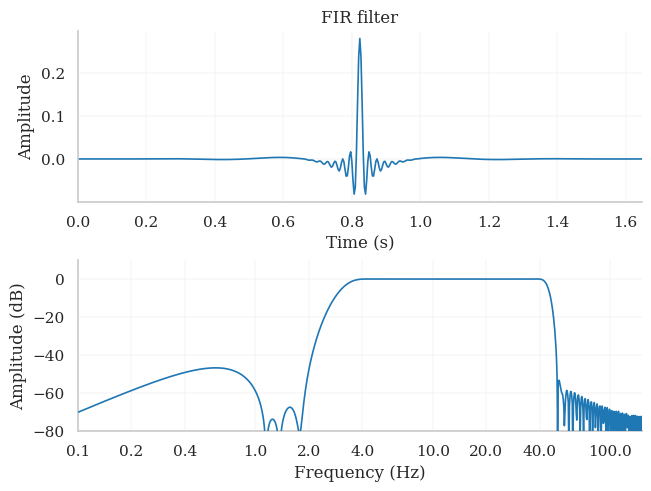
\includegraphics[width=12cm]{filtru.png}
    \caption{Filtrul bandpass folosit cu frecvențe între 4 și 40 Hz.}
		\vspace{-1em}
    \label{fig:vizualizare_filtru}
\end{figure}

Urmatoarea preprocesare aplicată este interpolarea canalelor corupte. Semnalul canalelor marcate ca fiind corupte este înlocuit prin interpolarea canalelor vecine acestuia. Mai departe, am aplicat tehnica de ICA(Independent Component Analysis) pentru a elimina clipirile din canalele Fp1 și Fp2 ce aveau reverberații și asupra celorlalte canale. Tehnica se bazează pe descompunerea semnalelor într-un număr de componente specificate. În contextul modului prin care am eliminat componentele legate de ochi, am implmentat două abordări. Prima este de a selecta manual componentele ce vrem să le eliminăm. Am făcut distincția dintre componentele ce trebuie păstrate și cele ce trebuie eliminate uitându-mă la rezultatul descompunerii și eliminând componentele ce au activări mai mari în zona ochilor. În exemplul din figura \ref{fig:descompunere_ica} acestea sunt: ICA002, ICA014 și ICA015. A doua abordare o reprezintă setarea unui prag de 2.5 deviații standard după care componentele să fie eliminate. În principal, componentele cele mai active sunt chiar cele din zona ochilor, acestea ajungând astfel să fie eliminate.
\begin{figure}[H]
    \centering
		\vspace{-1em}
    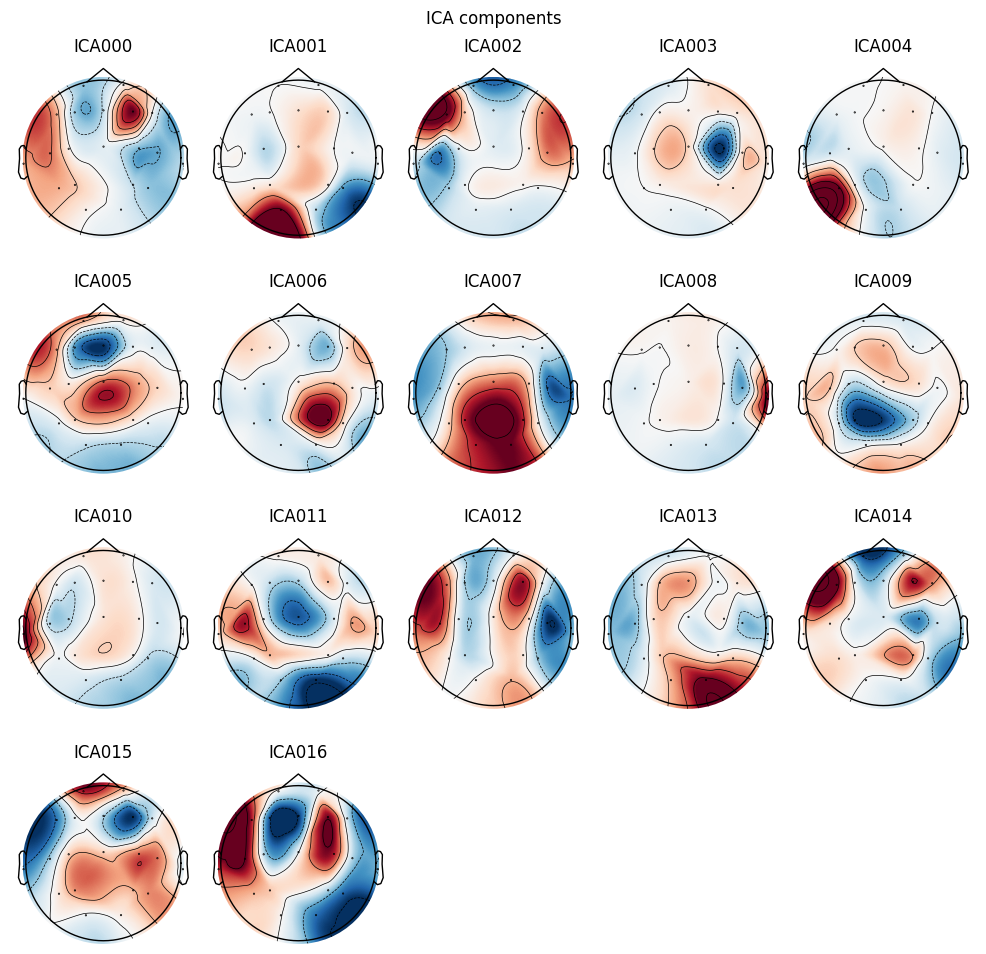
\includegraphics[width=8cm]{images/ica_components.png}
    \caption{Descompunerea ICA a semnalului.}
		\vspace{-1em}
    \label{fig:descompunere_ica}
\end{figure}

\begin{figure}[!htb]
    \centering
		\vspace{-1em}
    \begin{minipage}{\textwidth}
        \centering
        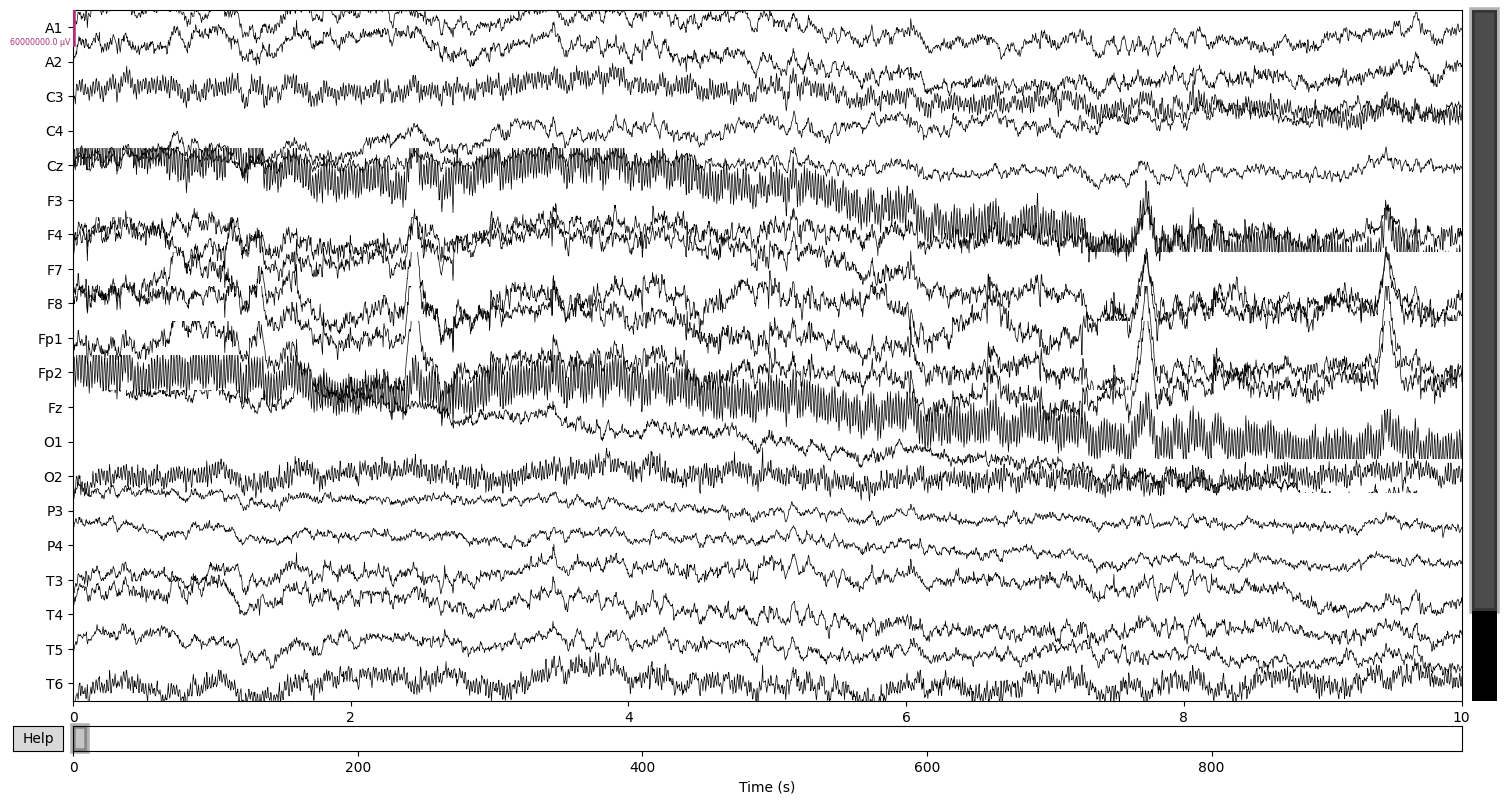
\includegraphics[width=0.8\textwidth]{images/raw_inainte.png}
        \label{fig:raw_inainte}
    \end{minipage}
    \vspace{0.5cm}
    \begin{minipage}{\textwidth}
        \centering
        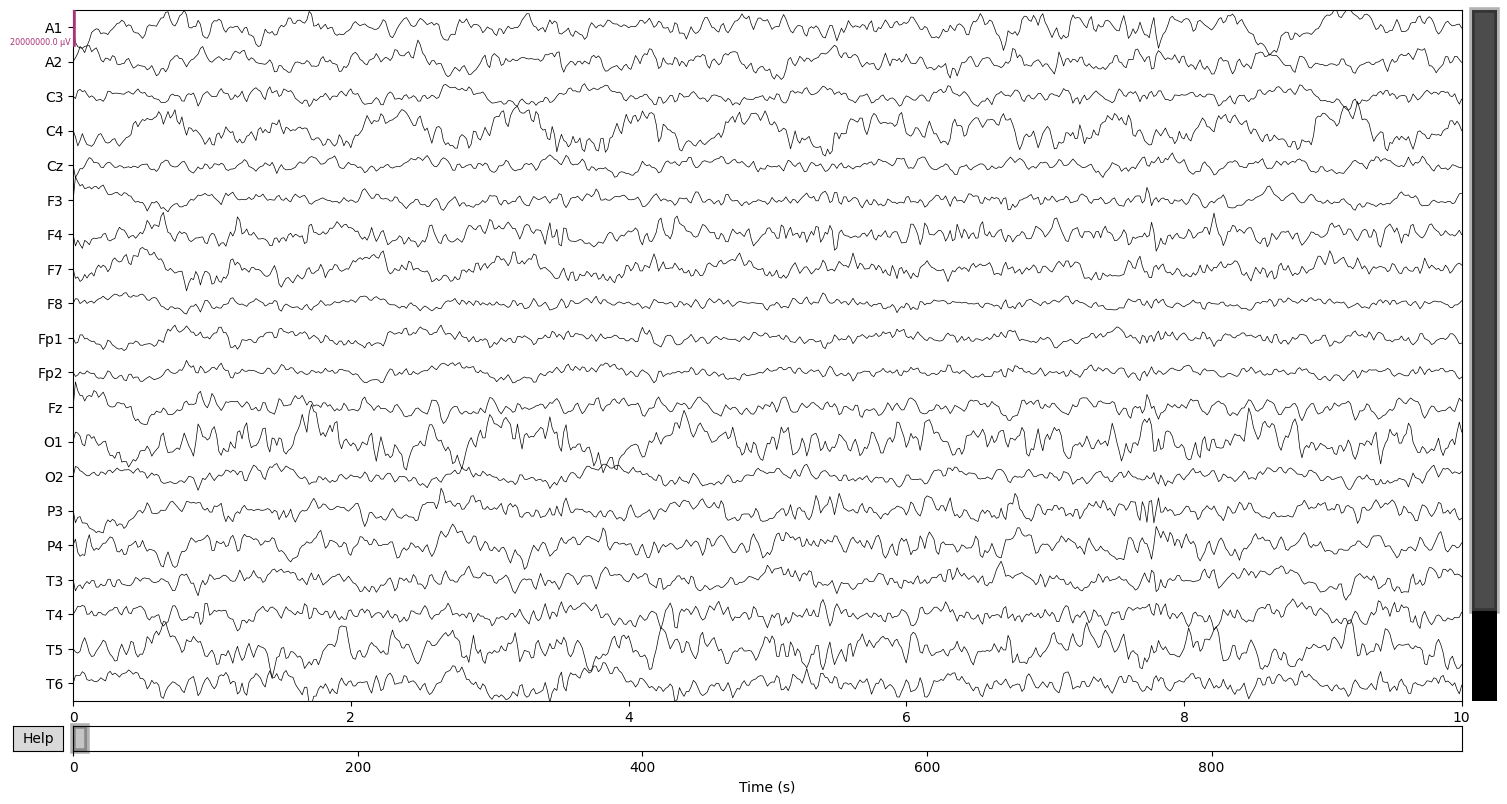
\includegraphics[width=0.8\textwidth]{images/raw_dupa.png}
        \label{fig:raw_dupa}
    \end{minipage}
    \caption{Semnalul înainte și după filtrare.}
		\vspace{-1em}
    \label{fig:raw_inainte_dupa}
\end{figure}

Calitatea datelor a fost semnificativ îmbunătățită. Am eliminat zgomotul cauzat de clipiri, drift-urile și frecvențele înalte.

\subsection{Separare în epoci, AutoReject}

Mai departe, pentru a avea date pentru clasificare, am împărțit semnalul continuu în epoci. O epocă reprezintă o fereastră mai mică din semnalul original. Aceasta este extrasă din semnalul continuu cu ajutorul unui canal auxiliar ce conține indexul stimulului prezentat sau 0 daca în acel moment nu este prezentat niciun stimul. Pentru a elimina eventualele probleme cauzate de mărimi diferite ale datelor, pentru fiecare epocă am luat și 0.2 secunde de semnal de dinaintea evenimentului de declanșare (afișarea imaginii). Această porțiune a fost folosită pe post de valoare de referință, valoarea acesteia fiind scăzută din restul semnalului. În acest fel, începutul și sfârșitul fiecărei epoci au fost centrate în jurul valorii zero. Figura \ref{fig:raspuns_mediu} ne confirmă atât faptul că începutul și sfârșitul epocilor sunt centrate corespunzător, cât și faptul că ICA a reușit să elimine activările din zona ochilor Fp1 și Fp2. Principalele activări se situează în zona O1, O2.

\begin{figure}[H]
    \centering
		\vspace{-1em}
    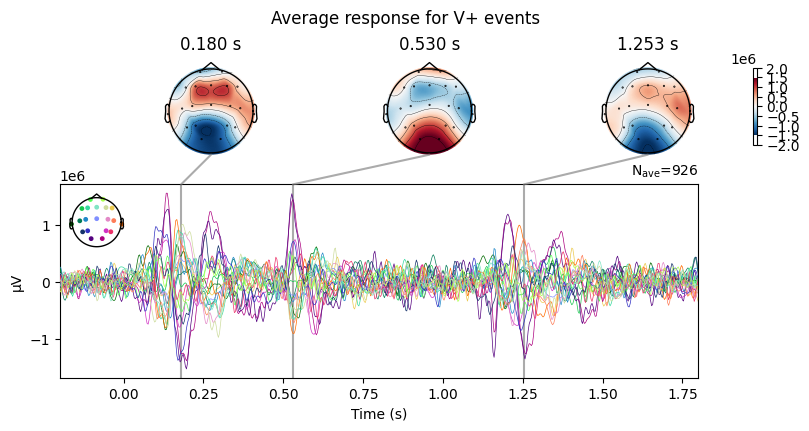
\includegraphics[width=13cm]{epoca_valenta_pozitiva.png}
    \caption{Raspunsul mediu al tuturor subiecților pentru o imagine cu valență pozitivă.}
		\vspace{-1em}
    \label{fig:raspuns_mediu}
\end{figure}

Totuși, nu toate epocile sunt bune. Unele dintre ele încă au imperfecțiuni și pot contamina datele de antrenare, așa că ele trebuie aruncate. Pentru a automatiza procesul de găsire și eliminare a epocilor corupte am folosit AutoReject\cite{AutoReject}. Această librarie găsește atât epoci corupte cât și canale corupte în epocile valide. AutoReject funcționează prin calcularea amplitudinii între vârfuri și văi (peek to peek amplitude) din cadrul unui semnal și selectarea anumitor praguri candidate. Algoritmul face acest lucru prin împărțirea epocilor în epoci de antrenare și testare, iar apoi folosește epocile de antrenare pentru a calcula pragul de eliminare, iar pe cele de testare pentru a calcula eroarea cauzată de acest prag. Eroarea este calculată între valoarea medie a setului de antrenare și mediana setului de testare folosind rădăcina mediei pătratului erorilor. Pragurile sunt alese dintr-un șir de praguri candidat.

Epocile selectate sunt eliminate complet, iar canalele considerate corupte sunt înlocuite prin interpolare. Impactul aplicării acestui proces a fost scăderea acurateții cu $\crestereAcurateteAutoReject$\%. Motivul pentru care performanța a scăzut este deoarece și datele de antrenare au scăzut semnificativ. Din figura \ref{fig:autoreject} reiese faptul că AutoReject găsește multe probleme în semnalul original. Există posibilitatea ca AutoReject să depisteze probleme exact acolo unde se află răspunsul creierului la stimul și prin urmare să scoată informația folositoare. Această teorie este susținută și de faptul că răspunsurile creierului nu sunt în conformitate cu restul semnalului. Figura \ref{fig:raspuns_mediu} ne indică faptul că amplitudinea semnalului în urma afișării stimulului este în afara mediei celorlalte canale. Prin urmare, AutoReject poate interpreta aceste vârfuri ca fiind date corupte.

\vspace{1em}
\begin{figure}[H]
    \centering
		\vspace{-1em}
    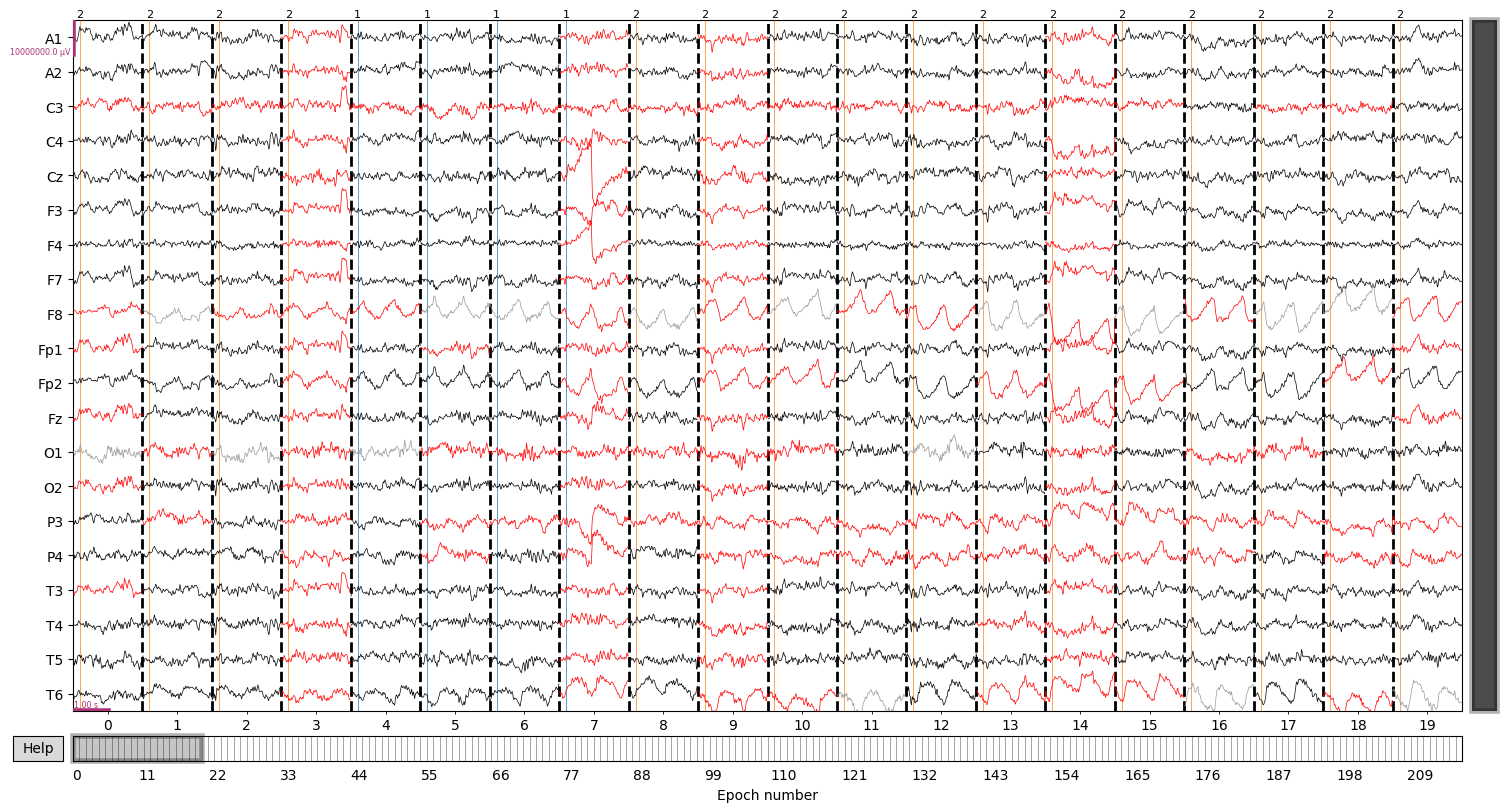
\includegraphics[width=0.7\textwidth]{images/rezultat_autoreject.png}
    \caption{Epocile și canalele marcate de AutoReject ca fiind corupte.}
		\vspace{-1em}
    \label{fig:autoreject}
\end{figure}

\subsection{Balansarea claselor și modul de testare}

În total am dispus de $\totalEpoci$ epoci provenite din cei 26 de subiecți. Din rândul tuturor epocilor, $\totalEpociValentaNegativa$ au valență negativă, $\totalEpociValentaNeutra$ neutră și $\totalEpociValentaPozitiva$ pozitivă. Numărul poate varia, deoarece AutoReject conține și componente non-deterministe. Pentru a testa performanța modelelor, am utilizat validarea încrucișată asupra celor 26 participanți în felul următor: $\nrParticipantiAntrenare$ de participanți au fost extrași pentru antrenare, $\nrParticipantiValidare$ pentru validare și încă $\nrParticipantiTestare$ pentru testare. În total am trecut prin câte 8 subseturi pentru fiecare model în parte.

Constatăm faptul că epocile nu sunt distribuite după etichetă în mod egal. Dacă modelul ar prezice numai valență neutră, ar avea acuratețe mai mare decât dacă ar prezice aleator. Pentru a aborda problema imbalansului claselor am folosit două abordări. Prima este de a calcula ponderile claselor, transmițându-le mai departe funcției de pierdere a clasificatorului. A doua este de a utiliza metoda numită Synthetic Minority Oversampling Technique (SMOTE)\cite{imblearn} pentru a genera date sintetice.

\section{Extragerea caractersiticilor}
În domeniul clasificării semnalelor EEG există 2 paradigme pentru extragerea caracteristicilor. Prima este de a trata semnalul EEG ca fiind o serie de timp. Datele de eșantioanare ale semnalului sunt trimise mai departe spre model ca input. În cele mai multe cazuri, modelele ce însoțesc această abordare sunt bazate pe rețele neuronale adânci, reprezentate de LSTM-uri, rețele convoluționale și transformere. A doua este de a extrage caracteristici statistice și geometrice din semnal. Acestea sunt sub forma de medii, proprietăți spectrale și caracteristici geometrice Riemann, care mai apoi sunt transmise unui model. Corespunzător acestei abordări sunt modelele mai simpliste, precum SVM-uri sau arbori de decizie, capabile de a separa liniar, folosind un număr mic de parametrii caracteristicile extrase. Contrar acestei observații, am încercat prima abordare inclusiv cu modele liniare, plecând de la ipoteza că reacția participanților se aseamănă între experimente de-a lungul celor trei categorii și produc răspunsuri neuronale asemănătoare ce ar avea poziții apropiate în spațiul de separare.


\subsection{Datele drept semnale EEG}
După cum am spus, semnalul EEG are 20 de canale. Totuși, dintre acestea, nu toate sunt relevante. Pentru a găsi cele mai relevante canale, în primul rând am transpus semnalul in domeniul timp-frecvență utilizând implementarea din MNE\cite{MNE} a undelor Morlet. Am aplicat această operație pentru toate epocile și, astfel, am obținut coerența inter-experiment(ITC, sau inter-trial coherence). ITC ul îmi arată asemănarea în descompunerea din domeniul timp-frecvență a epocilor.

\begin{figure}[H]
    \centering
		\vspace{-1em}
    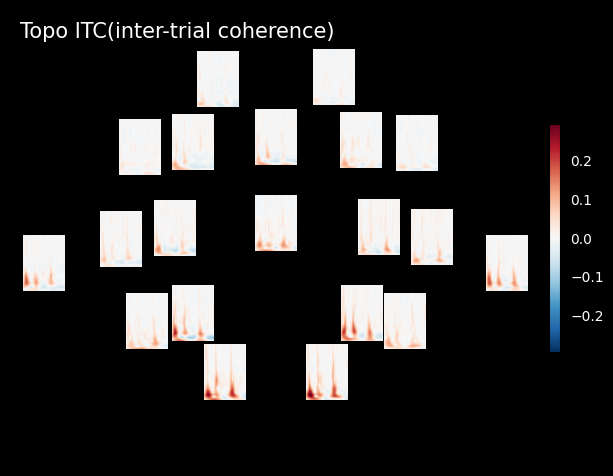
\includegraphics[width=0.6\textwidth]{images/itc_epochs.png}
    \caption{ITC-ul de-a lungul tuturor epocilor înregistrate pentru toți participanții.}
		\vspace{-1em}
    \label{fig:itc}
\end{figure}

Putem remarca faptul că diagrama \ref{fig:itc} are o dispunere asemănătoare cu cea a plotării electrozilor pe creier, figura \ref{fig:sensor_positions}. Din această diagramă observăm importanța fiecărui canal în timpul unei epoci. Astfel, de exemplu, canalele Fp1 și Fp2 nu oferă la fel de multă informație comparativ cu O1 sau O2. Canalele alese de mine ca fiind relevante au fost: O1, O2, P3, P4, A1, A2, T5, T6. Alegând un subset de canale din cele inițiale, am mărit viteza cu care am procesat datele cu 36\%, precum și acuratețea modelului cu 3-4\%.

\vspace{1em}
\begin{figure}[H]
    \centering
		\vspace{-1em}
    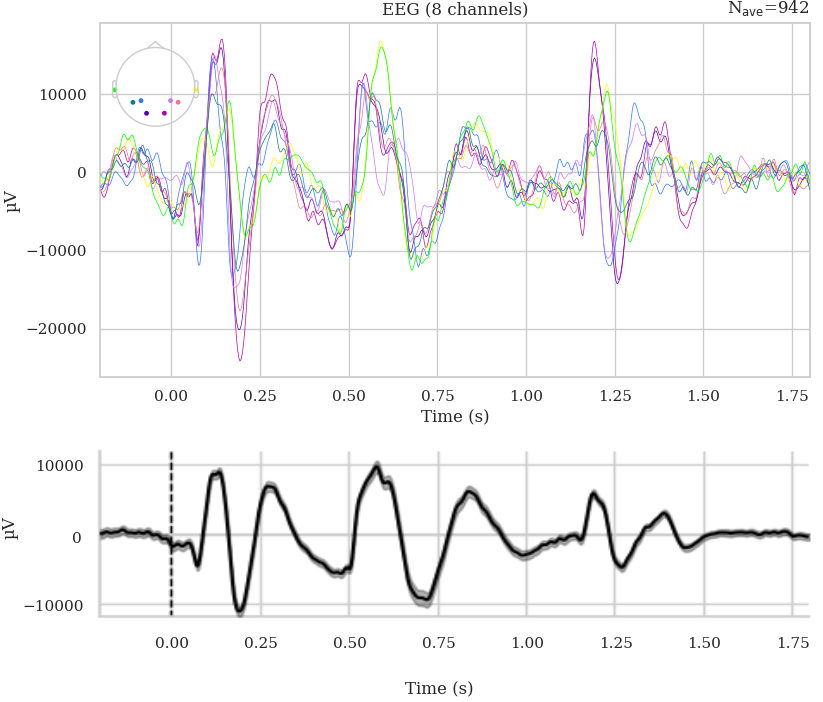
\includegraphics[width=1\linewidth, height=10cm, keepaspectratio=false]{P300_combined.png}
    \caption{ERP-ul canalelor selectate O1, O2, P3, P4, A1, A2, T5, T6.}
		\vspace{-1em}
    \label{fig:enter-label}
\end{figure}

Un alt rezultat al alegerii unui subset de canale a fost faptul că, am reușit să apropii evenimentul de unul de tip P300\cite{P300}, fiind bine cunoscut și studiat în neuroștiință. Teoria spune că, odată prezentat un stimul unui participant, răspunsul cognitiv apare la aproximativ 300 de milisecunde după evenimentul declanșator. În cazul meu, observăm că aproximativ după 0.3 s de la afișarea stimulului (momentul 0) apare un vârf, fiind precedat și antecedat de 'văi'. Prima vale are denumirea de P200, iar a doua de P300. Această dispunere a semnalului confirmă faptul că preprocesările făcute nu au alterat semnificația semnalului. %În plus, dispunerea semnalului sub forma P300 mi-a permis sa abordez și metode de transfer-learning pe seturi mai mari de date și cu mai mulți electrozi.

\vspace{1em}
\begin{figure}[H]
    \centering
		\vspace{-1em}
    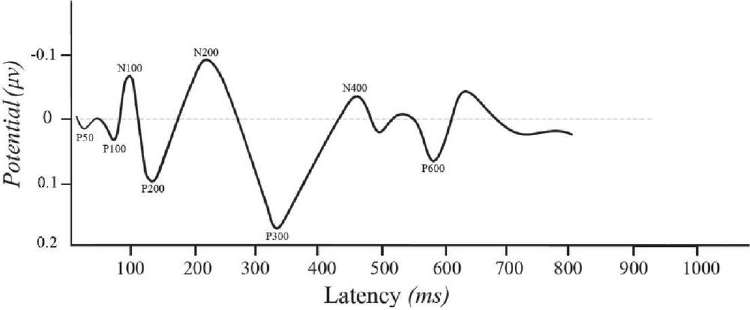
\includegraphics[width=0.9\linewidth]{P300_theory.jpg}
    \caption{Evenimentele asociate unui ERP\cite{P300_image}.}
		\vspace{-1em}
    \label{fig:enter-label}
\end{figure}

Am confirmat că într-adevăr există diferențe între fiecare tip de stimuli unind toți participanții și realizând în Appendix un grafic al mediei răspunsurilor celor trei tipuri de stimuli. Graficul poate fi văzut în figura \ref{fig:average_response_by_event} din Appendix.

\subsection{Datele drept caracteristici statistice și descompuneri în domeniul frecvențelor}

O altă abordare a extragerii caracteristicilor o reprezintă datele statistice și spectrale din semnalul EEG. Pentru a extrage caracteristicile semnalului am utilizat mne-features\cite{mne-features}. Librăria reușește să extragă în total 30 de tipuri de caracteristici. Am restrâns aceste caracteristici la o submulțime mai mică, implementând metoda prezentată în \cite{ga_svm}. Și anume folosirea algoritmilor genetici împreuă cu un clasificator liniar SVM pentru a alege o submulțime de caracteristici din cea inițială. 

\subsection{Datele drept caracteristici geometrice Riemann}
Alte modalități, care au recâștigat popularitate recent, constau în folosirea geometriei Riemann. În domeniul semnalelor EEG, o caracteristică importantă o reprezintă matricile de covarianță. Acestea indică impactul unui canal asupra celorlalte canale. O matrice de covarianță este o matrice pătratică, având canalele dispuse pe verticală și orizontală. Pe diagonala principală valorile indică varianța unui canal față de meida sa, iar în afara diagonalei matricea indică influența unui canal asupra altui canal. Daca un astfel de coeficient de covarianță este pozitiv, înseamnă că semnalele se mișcă în același sens, iar dacă este negativ se mișcă în sens opus. Este dovedit faptul că aceste matrici sunt simetrice și pozitiv definite (SPD). Astfel, spațiul din care provin ele nu este unul euclidian ci unul cu neliniar, curbat, și anume spațiul Riemann. Prin urmare, transpunerea din spațiul euclidian în spațiul Riemann are efectul de a reintroduce caracteristicile pierdute din 'aplatizarea' spațiului din care provin matricile de covarianță \cite{riemann_geometry}.

Asupra datelor este aplicat algoritmul de denoising XDAWN\cite{xdawn}, urmând, pe urmă, ca semnalul să fie transpus într-un spațiu geometric Riemann. Pentru a implementa acești algoritmi m-am folosit de librăria pyRiemann\cite{pyriemann}. Algoritmii ce se folosesc de acest principiu și pe care i-am implementat și testat la rândul meu sunt: XDAWNCov + TS + SVM\cite{xdawncovtssvm}, pe care ulterior l-am modificat si am utilizat Linear Discriminant Analysis(LDA) din scikit-learn\cite{scikit-learn}, XDAWN + LDA\cite{xdawnlda}, și, derivat din aceste concepte XDAWN + Cov + TS + LDA. Benchmark-urile MOABB\cite{moabb}  arată că XDAWNCov + TS + SVM și XDAWNCov + MDM obțin cele mai bune performanțe pentru stimulii de tip P300. Rezultatele obținute de mine sunt vizibile în figura \ref{fig:rezultate_xdawn}.

\vspace{1em}
\begin{figure}[H]
    \centering
		\vspace{-1em}
    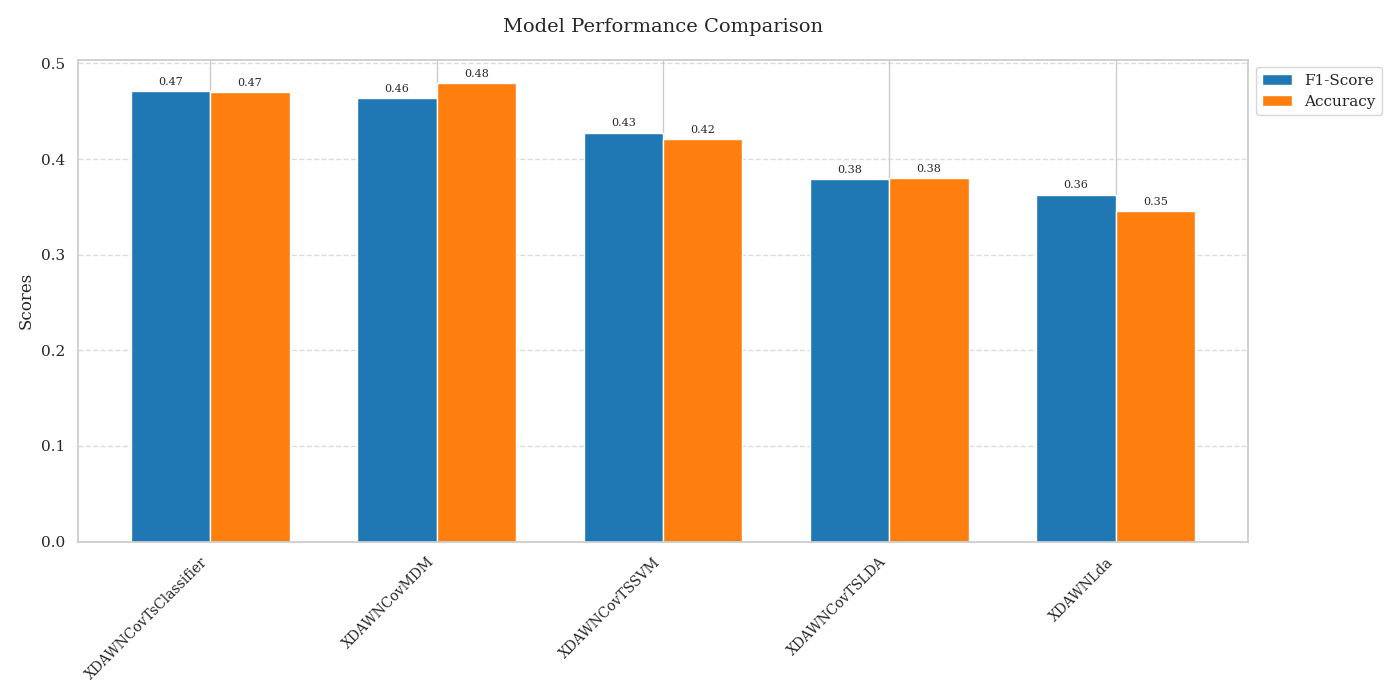
\includegraphics[width=1\linewidth]{comparison_xdawn.png}
    \caption{Comparație a performanțelor algoritmilor XDAWN.}
		\vspace{-1em}
    \label{fig:rezultate_xdawn}
\end{figure}

\section{Modele de clasificare}
Privind abordarea modelelor am ales să încerc cât mai multe modele, pornind de la simple clasificatoare liniare, precum SVM-uri din scikit-learn\cite{scikit-learn} și până la rețelele convoluționale din braindecode\cite{braindecode}. De asemenea, am creat, utilizând keras\cite{keras}, și modele proprii pentru un mai bun control asupra complexității și funcționalității modelului.
\subsection{Modele clasice din scikit-learn}
Pentru a evalua modelele clasice, prima dată am trecut datele de dimensiune(8, 601) adică 8 canale, fiecare canal având 601 puncte de discretizare, aceste 601 puncte provin de la frecvența înregistrărilor de 300 x 2 secunde ce reprezintă durata unei epoci, prin operația de flatten, astfel încât input-ul meu să fie 1-dimensional. Pe urmă, am normalizat datele și le-am încadrat în intervalul (0, 1) utilizând StandardScaler din scikit-learn\cite{scikit-learn}. În final, fiecare input reprezintă un vector cu 4808 caracteristici.

% \setlength{\abovecaptionskip}{0pt}
% \setlength{\belowcaptionskip}{0pt}
% \clearpage
% \begin{figure}[h]
%     \centering
%     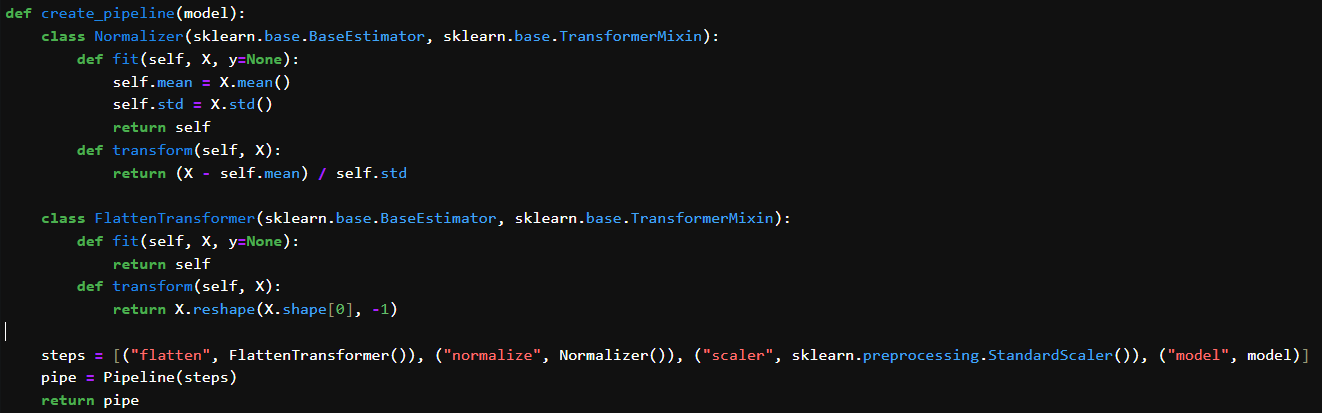
\includegraphics[width=1\linewidth]{pipeline_modele_clasice.png}
%     \caption{Pipeline pentru modelele clasice}
%     \label{fig:enter-label}
% \end{figure}

Utilizând acest pipeline, ce poate fi observat și în figura \ref{fig:pipeline_modele_clasice} din Appendix, am putut să compar sistematic mai multe tipuri de modele. Pentru a evalua performanța modelelor, am utilizat f1-score și accuracy. Pentru a lua în calcul imbalansul claselor, am creat date sintetice utilizând metoda de oversampling SMOTE\cite{imblearn}. %Pentru cel mai bun model din punctul de vedere al f1-score și accuracy am făcut mai departe un classification report. %

\vspace{1em}
\begin{figure}[H]
    \centering
		\vspace{-1em}
    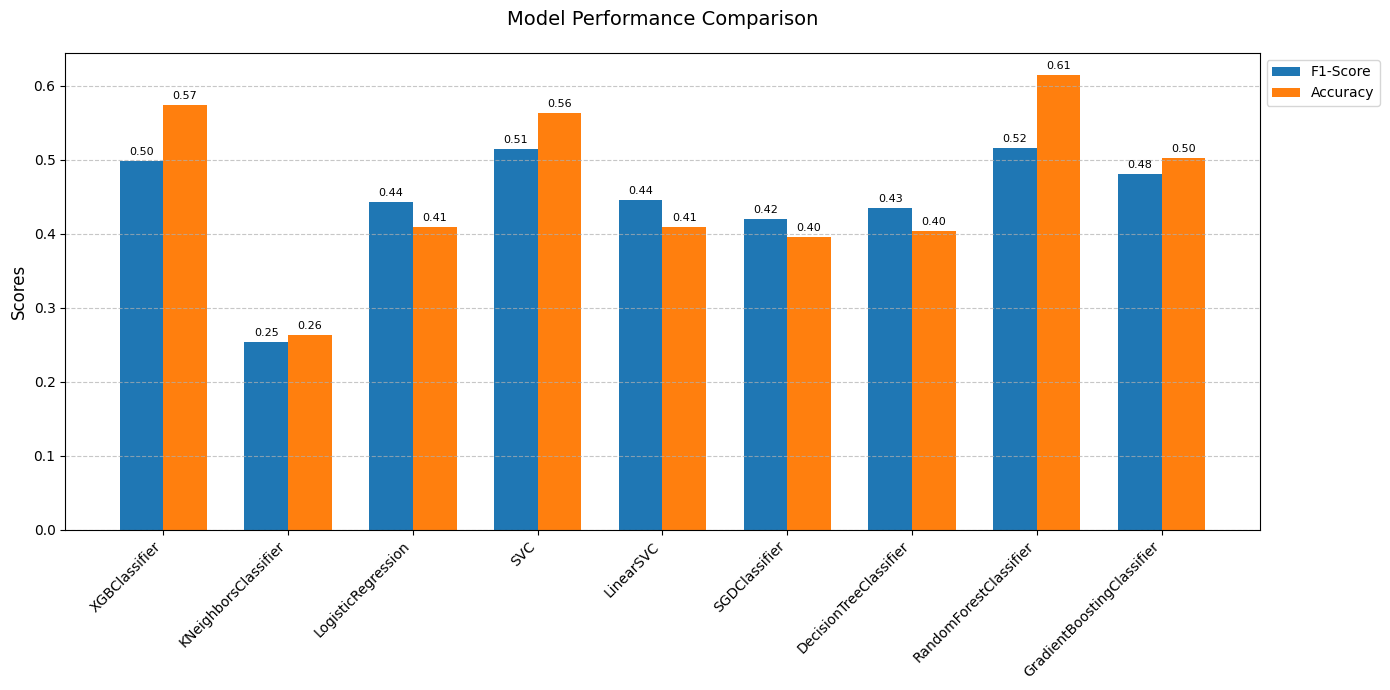
\includegraphics[width=1\textwidth]{images/comparatie_modele_clasice_unweighted.png}
    \caption{Comparație a performanțelor modelelor clasice din scikit-learn\cite{scikit-learn}.}
		\vspace{-1em}
    \label{fig:enter-label}
\end{figure}

Mai departe, în scopul de a implementa abordarea bazată pe caracteristici statistice și spectrale, am utilizat mne-features\cite{mne-features}. Pentru a extrage un subset din feature-urile totale, am utilizat o librărie specializată în rularea algoritmilor genetici, și anume pygad \cite{pygad}. Funcția de fitness a fost calculată folosind un tuplu format din f1-score și balanced-accuracy. Configurația specifică poate fi văzută în figura \ref{fig:pygad_configuration} din Appendix.

Un rezultat intermediar a indicat o acuratețe de 35\% și un scor F1 de 38\%. Având în vedere performanțele modeste și dimensiunea ridicată a spațiului de căutare, am decis să întrerup rularea experimentului în această configurație. Continuarea optimizării în aceste condiții nu era justificată, întrucât rezultatele obținute nu indicau un potențial de îmbunătățire semnificativă. Rezultatele lucrării care implementeaza această idee \cite{ATKINSON201635}, indică faptul că algoritmul genetic a făcut ca acuratețea să varieze cu un maxim de 5\%, rezultat care în continuare l-ar plasa sub performanța celorlalte modele încercate. 

\subsection{Braindecode}
Pentru a avea acces la arhitecturi neuronale avansate, create special pentru domeniul analizei EEG-urilor, am utilizat librăria Braindecode\cite{braindecode}. Ele primesc drept intrare direct semnalul de dimensiune (8, 601). Fiecare model din braindecode trebuie trimis mai departe unui wrapper, fie de regresie fie de clasificare. Apelul wrapper-ului poate fi văzut în figura \ref{fig:wrapper_braindecode} din Appendix. În cazul meu l-am folosit pe cel de clasificare. Pentru a mări viteza de procesare, dispunând de o placă video, am rulat antrenarea epocilor pe placa video folosind cuda.

La nivelul acestuia am setat funcția de pierdere ca fiind CrossEntropyLoss din librăria pytorch \cite{pytorch}, precum și EarlyStopping și LRScheduler drept callback-uri din librăria skorch \cite{skorch}. Astfel, modelul evită overfitting-ul prin oprirea antrenării în momentul în care nu a mai progresat din punctul de vedere al funcției de pierdere pe setul de validare timp de 20 de epoci. De asemenea, acesta dispune și de un learning rate variabil ce îl ajută sa conveargă rapid la o soluție. 

\begin{equation}
    \text{loss}(x, y) = -\frac{1}{N} \sum_{n=1}^{N} w_{y_n} \cdot \log\left(\frac{\exp(x_{n,y_n})}{\sum_{c=1}^{C} \exp(x_{n,c})}\right) \times \mathbb{1}\{y_n \neq \text{ignore\_index}\}
\end{equation}

Putem remarca faptul că formula pentru CrossEntropyLoss conține un \(w_{y_n}\). Acesta reprezintă un parametru legat de imbalansul claselor. Astfel, modelul îmi permite să abordez ambele modalități de rezolvare a problemei de balansare a claselor. Evaluarea modelelor am făcut-o asemănător cu cea a modelelor clasice, în funcție de f1-score și accuracy.

Cu scopul de a avea o analiză amplă a acestei tehnici, am utilizat toate modelele disponibile din librărie ce au fost dezvoltate în direcția interpretării evenimentelor de tip P300. Astfel, am comparat următoarele modele: TSceptionV1\cite{TSception}, EEGNetv4\cite{eegnetv4}, EEGInceptionERP\cite{eeginceptionerp}, ATCNet \cite{atcnet1}\cite{atcnet2}\cite{atcnet3}, EEGTCNet\cite{tcnet}, TIDNet\cite{tidnet}, ShallowFBCSPNet\cite{ShallowFBCSPNet}.

De asemenea, am creeat noi date folosind augmentări,. Observând că studii din trecut au obținut rezultate mai bune după ce le-au aplicat \cite{Wang2018}. Augmentările folosite au fost: deplasarea întregului semnal cu până la 20 de secunde înainte și înapoi, zgomot gaussian, și setarea semnalului la valoarea 0 pentru diverse perioade. Codul cu care am realizat augmentările poate fi văzut în Appendix în figura \ref{fig:augmentari}.

\vspace{1em}
\begin{figure}[H]
\begin{center}

\end{center}
    \centering
		\vspace{-1em}
    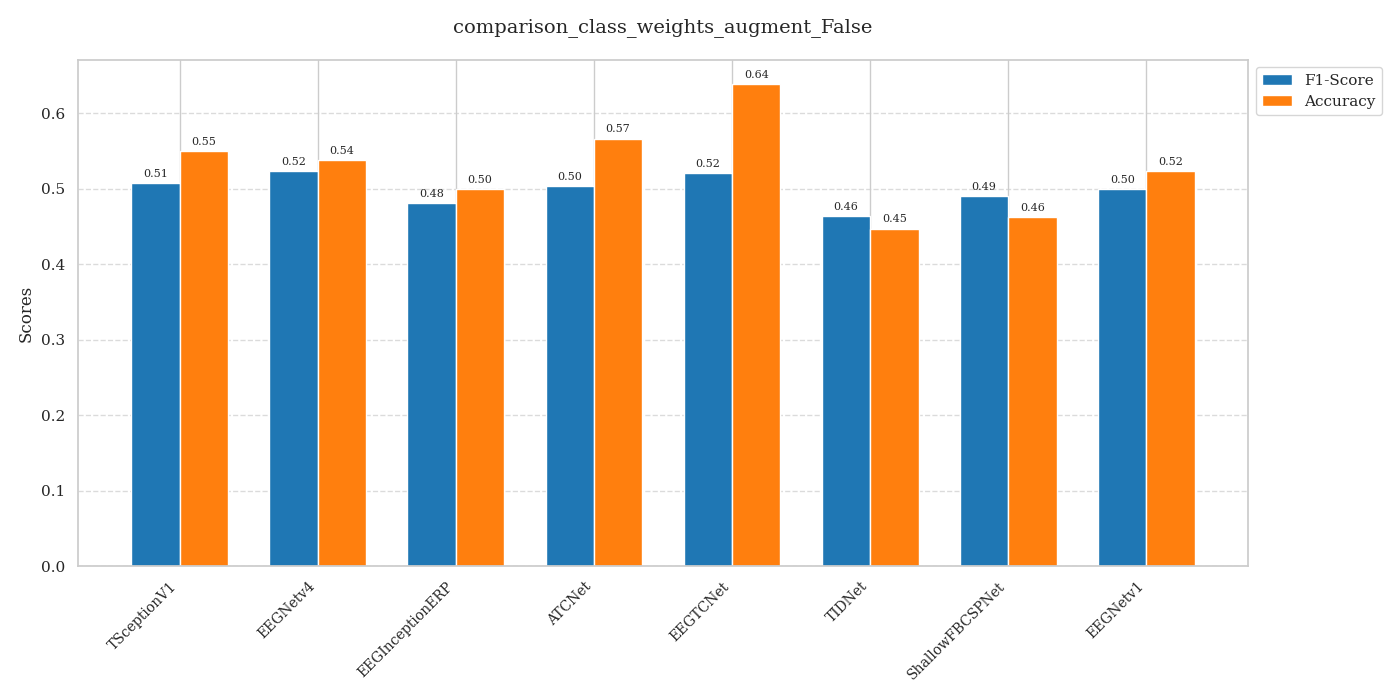
\includegraphics[width=1\textwidth]{images/comparison_class_weights_augment_False.png}
    \caption{Comparație a performanțelor modelelor din braindecode\cite{braindecode}.}
		\vspace{-1em}
    \label{fig:performanta_braindecode}
\end{figure}

Este evident din figura \ref{fig:performanta_braindecode}, faptul că EEGTCNet\cite{tcnet} a obținut cele mai bune rezultate. Acestea au fost obținute atunci când modul de tratare a imbalansului claselor a constat în calcularea weight-urilor claselor, trimis mai departe la funcția de pierdere și atunci când nu au fost aplicate augmentări pe date. Rezultatul celorlalte abordări privind imbalansul claselor și augmentări se află în figurile \ref{fig:performance_class_weights_augment_true}, \ref{fig:smote_augment_false} și \ref{fig:smote_augment_true} din Appendix.


\subsection{Model personal}
Am creeat modele personale utilizând librăria Keras\cite{keras}. Am ales să folosesc această bibliotecă în defavoarea PyTorch, deoarece Keras oferă un nivel mai ridicat de abstractizare, ceea ce simplifică considerabil procesul de dezvoltare a modelelor. Un alt motiv pentru care am utilizat Keras este faptul că pașii de antrenare, optimizare și validare sunt deja integrați și gestionați bine de bibliotecă. În contextul acestei lucrări, nu a fost necesară personalizarea acestor pași sau implementarea unor mecanisme avansate de calculare a funcției de pierdere sau de control de date. 

Paradigma pe care am abordat-o a fost cea în care trimit modelului semnalul în sine, urmând ca în cadrul modelului să extragem proprietăți ale semnalului folosind rețele convoluționale. Arhitectura modelului meu constă în 3 straturi de convoluție, între ele aflându-se straturi de MaxPooling. La final am aplatizat rezultatul convoluțiilor și am terminat modelul cu 3 straturi dense. Pentru a preveni problem overfitting-ului am aplicat regularizarea L1 și L2, am introdus dropout în straturile dense și am augmentat datele la intrarea în model cu zgomot gausian. Drept optimizator am folosit Adam. Neuronilor de output le-am aplicat funția de activare softmax pentru a fi compatibil cu funcția de pierdere CategoricalCrossEntropyLoss. Pentru restul neuronilor am utilizat funcțiile de activare ReLU și ELU. Arhitectura modelului detaliată este reprezentată în figurile \ref{fig:model_part1} și \ref{fig:model_part2} din Appendix.

\begin{figure}[H]
    \centering
		\vspace{-1em}
    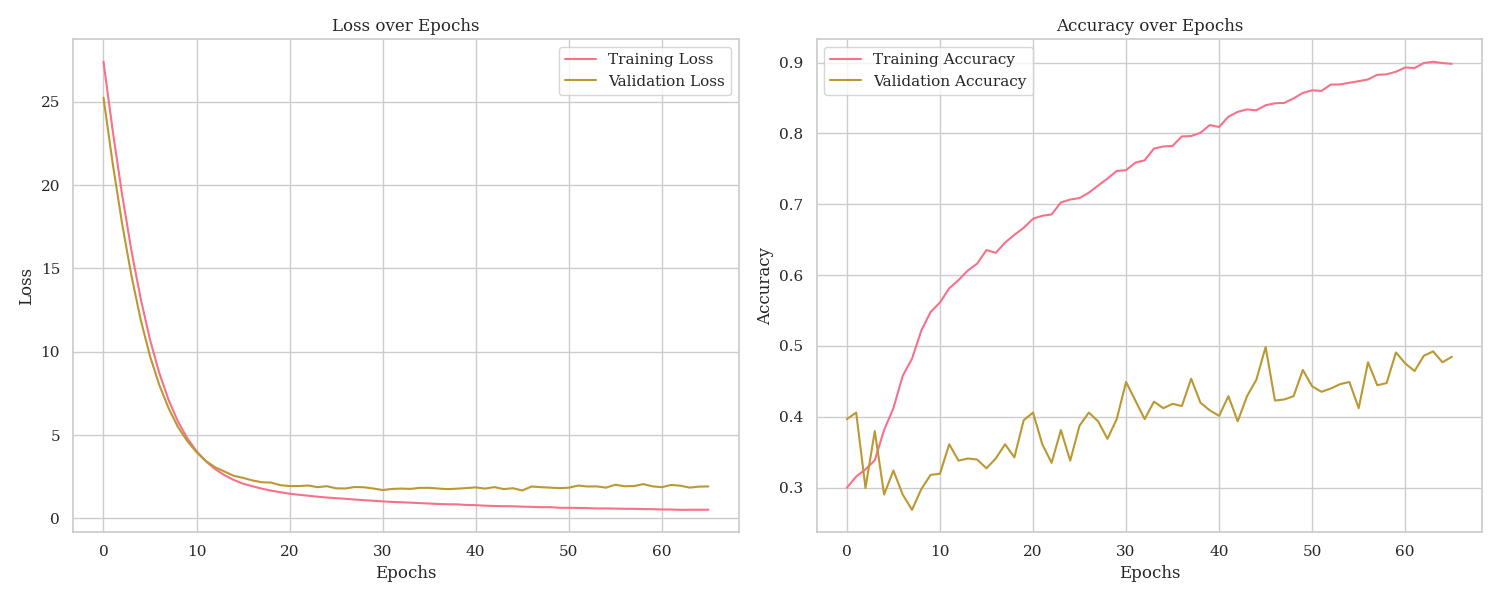
\includegraphics[width=1\linewidth]{images/comparison_fold7.png}
    \caption{Evoluția funției de pierdere și a acurateții de-a lungul epocilor.}
		\vspace{-1em}
    \label{fig:model_train}
\end{figure}

Figura \ref{fig:model_train} ne arată evoluția funcției de pierdere, precum și a acurateții modelului pe parcursul epocilor. Putem observa că modelul reușește să învețe până ajunge la o acuratețe de sub 50\%. În evaluarea finală în care am combinat toate rezultatele din urma validării în cruce a modelul am obținut o acuratețe de 47\%. Din matricea de confuzie prezentată în figura \ref{fig:conf_matrix} observăm că modelul în continuare are o predispoziție în a prezice valența neutra (2).

\begin{figure}[H]
    \centering
		\vspace{-1em}
    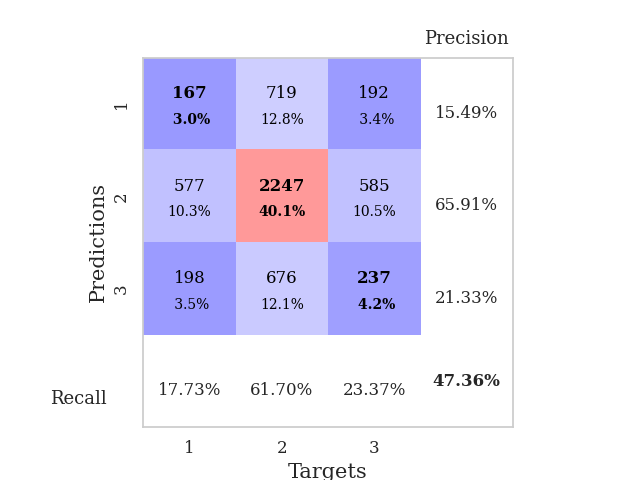
\includegraphics[width=0.7\linewidth]{conf_matrix_personal_model.png}
    \caption{Matricea de confuzie rezultată în urma validărilor.}
		\vspace{-1em}
    \label{fig:conf_matrix}
\end{figure}

Lipsa capacității modelului de a învăța diferențe clare între clase poate fi atribuită metodelor de balansare a acestora. În cazul balansării prin calcularea weight-urilor, modelul acordă o importanță mai mare instanțelor în care subiecții au spus că le place/ nu le place imaginea (acestea fiind cele mai rare). Astfel, deși modelul ajunge să învețe bine exemplele din timpul antrenării, performanța sa pe date noi scade, întrucât răspunsul creierului variază semnificativ atât în intensitate, cât și în timp. Punând un accent mai mare pe exemplele rare dintr-un set de date limitat ca dimensiune, modelul nu reușește să surprindă variabilitatea naturală a activității cerebrale nici la nivel intra-subiect (același participant), nici inter-subiect (între participanți diferiți).


Fenomenul acesta este observat și în cadrul balansării folosind SMOTE\cite{imblearn}. Algoritmul de generare al datelor sintetice încearcă să umple golul dintre sample-uri prin interpolare. Totuși, aceste instanțe nu introduc informație nouă, ci doar reflectă o medie a celorlalte doua puncte din vecinătatea exemplului sintetic. Mecanismul de generare de date sintetice nu reproduce modul natural de funcționare al creierlului uman. Chiar și in condiții de expunere repetată la același stimul, variația răspunsului cerebral nu este rezultatul unei medii liniare între două stări, ci al unui proces complex de interpretare și adaptare.
%\chapter{Rezultate}

\section{Evaluarea performantei}
\subsection{Metrici utilizate: acuratetea, precizie, f1-score}

\section{Analiza detaliata a rezultatelor}
\subsection{Compararea performantelor intre diferite modele(graficele mele)}

\section{Grafice si interpretarea acestora}
\subsection{Curbe ROC, matricea de confuzie, etc.}

\def\timpInainteDeRay{37}
\def\timpDupaRay{18}

\chapter{Arhitectura aplicației}
\section{Împărțirea codului}
Codul este împărțit în 4 clase diferite. Ele au rolul de a forma un pipeline ce primește la intrare fișiere în format csv, împreună cu montura electrozilor și ca rezultat oferă obiecte în formatul librăriei MNE\cite{MNE}.
În total, pipeline-ul meu este format din 5 clase: EEGPipelineOptions, EEGSubjectPipeline, EEGDataLoader, EEGPreprocessor și EEGEpochedData. 

Prima dată, opțiunile de preprocesare și de formatare în epoci sunt setate utilizând EEGPipelineOptions. Acest obiect este trimis mai departe către EEGSubjectPipeline. Aici, este orchestrat restul pipeline-ului în felul următor: datele din format .csv sunt transformate în format .fif(compatibil cu MNE\cite{MNE}) utilizând EEGDataLoader. Datele în format .fif sunt transformate în date de forma mne.Raw, reprezentând semnalul întreg, nesegmentat în ferestre ERP. Aici sunt totodată și preprocesate utilizând filtrul trece-bandă, ICA, interpolarea, și/sau, opțional, normalizare și scalare în intervalul [0, 1].  Ultimul pas îl reprezintă EEGEpochedData, unde semnalul Raw este segmentat în epoci. În funcție de opțiunile alese, aici poate fi aplicat și algoritmul de AutoReject\cite{AutoReject} pentru a elimina epocile corupte. Totodată, în această clasă este situată și funcția de extragere a setului de date, împreună cu etichetele acestuia.


\section{Alte librării folosite}
\subsection{Optimizarea încărcării datelor folosind Ray}
Pentru a încărca eficient cei 26 de participanți am utilizat librăria Ray\cite{Ray}. Ray este o librărie specializată în paralelizarea programelor Python, având ca scop principal programele din domeniul de Machine Learning. Modul de paralelizare a constat în decorarea funcțiilor de încarcare a datelor cu @ray.remote și așteptarea rezultatului cu ray.get. Timpul de încărcare a datelor participanților a fost redus de la $\timpInainteDeRay$ secunde la $\timpDupaRay$ secunde. Paralelizarea folosind Ray poate fi observată în figura \ref{fig:paralelizare_ray} din Appendix. Această scădere a avut un impact accentuat în momentul căutării hiperparametrilor, am putut astfel să dublez totalul parametrilor căutați în același interval de timp.

%După cum putem observa în figura \ref{fig:load_calculator}, paralelizarea a funcționat, ducând procesorul calculatorului la 100\%.

\subsection{Căutarea hiperparametrilor folosind Optuna}
Optuna\cite{optuna_2019} este o librărie ce se ocupă de căutarea hiperparametrilor. Parametrii căutați au fost cei legați de EEGPipelineOptions. Scopul a fost să înțeleg ce preprocesări trebuiesc executate pentru performanță maximă. Pentru a rula pipeline-ul meu folosind optuna, am definit o funcție obiectiv, și anume f1 score-ul obținut în urma validării încrucișate. Mai departe, am setat hiperparametrii pe care ar trebui să-i caute librăria. Am salvat cei mai buni parametrii în funcție de scorul F1. Astfel, am putut să caut sistematic cei mai buni hiperparametrii de preprocesare. Întreg procesul poate fi văzut în detaliu în figura \ref{fig:optuna_search} din Appendix.

\chapter{Concluzii}

\section{Interpretarea rezultatelor}

Observând rezultatele obținute, am ajuns la concluzia că stimulii nu au fost destul de puternici astfel încât să existe o distincție clară între reacția subiecților la aceștia. Iar, dacă privim literatura de specialitate în domeniul EEG-urilor, și în special pe cel al clasificării emoțiilor, putem observa rezultate cel mult medicore\cite{recreation_attempt}, chiar și pe seturi de date bine cunoscute. Încercând cât mai multe lucruri și citind lucrări de specialitate am observat că există destule limitări în acest domeniu. Multe dintre limitări sunt legate de metodele de recoltare a datelor și de zgomotul rezultat de acestea, altele sunt legate de diferențele fiziologice dintre oameni, neputând astfel generaliza un stimul unifrom de-a lungul unor subiecți. O analiză mai amplă și precisă poate fi facută, momentan, folosind tehnologie non-invazivă, doar pe stimuli de durată mai lungă, unde cel mai important factor este frecvența, sau stimuli mai puternici și mai diverși. 

\section{Îmbunătățiri și perspective de viitor}

Pentru a îmbunătăți rezultalte, experimentul ar putea fi realuat folosind imagini mai stimulante, afișate pe o perioadă mai lungă de timp. De asemena, încă o îmbunătățire ar putea fi adusă și prin folosirea unui eyetracker, astfel combinând reacția, cu zona în care s-a uitat participantul când a avut-o. În plus, un alt aspect care ar putea îmbunătăți rezultalte, ar fi creșterea gradului de imersiune folosind, de exemplu, căști de realitate virtuală.

\printbibliography[heading=bibintoc]

\appendix
\chapter{Tabele cu rezultate}

\begin{figure}
    \centering
    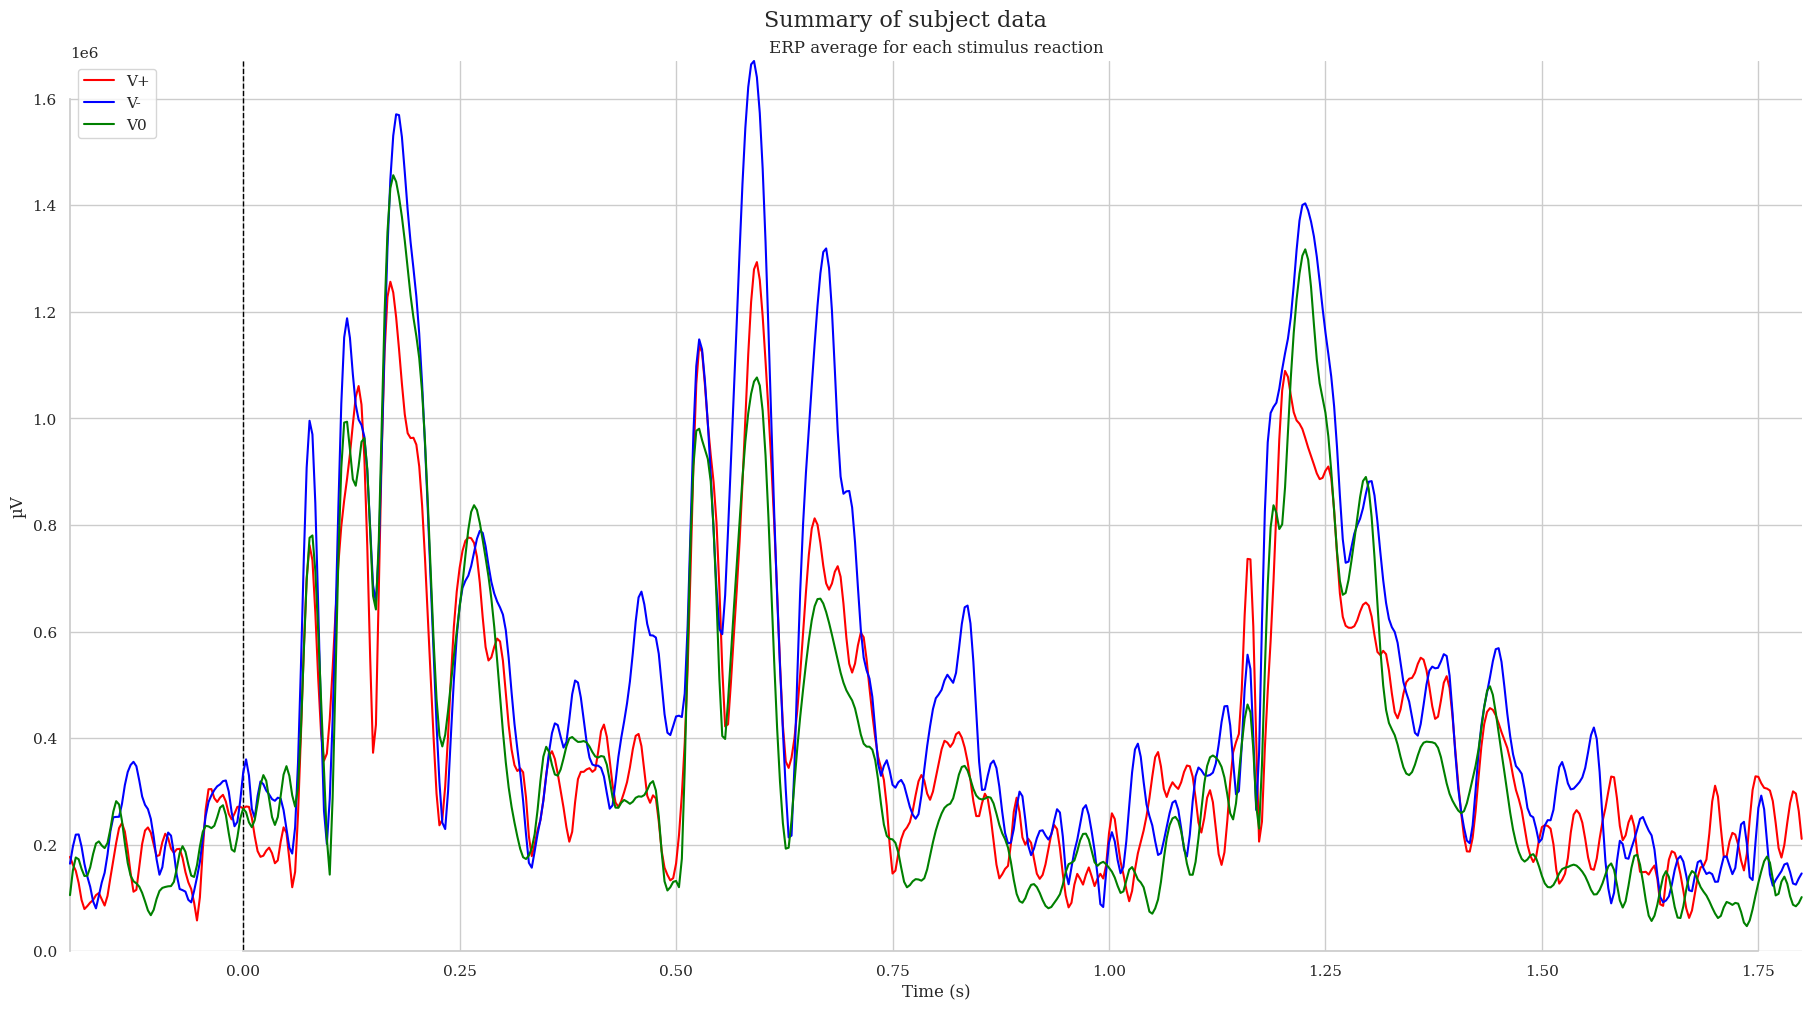
\includegraphics[width=1\linewidth]{images/average_response_each_erp.png}
    \caption{Răspunsul mediu pentru fiecare tip de eveniment.}
    \label{fig:average_response_by_event}
\end{figure}

\begin{figure}[h]
    \centering
    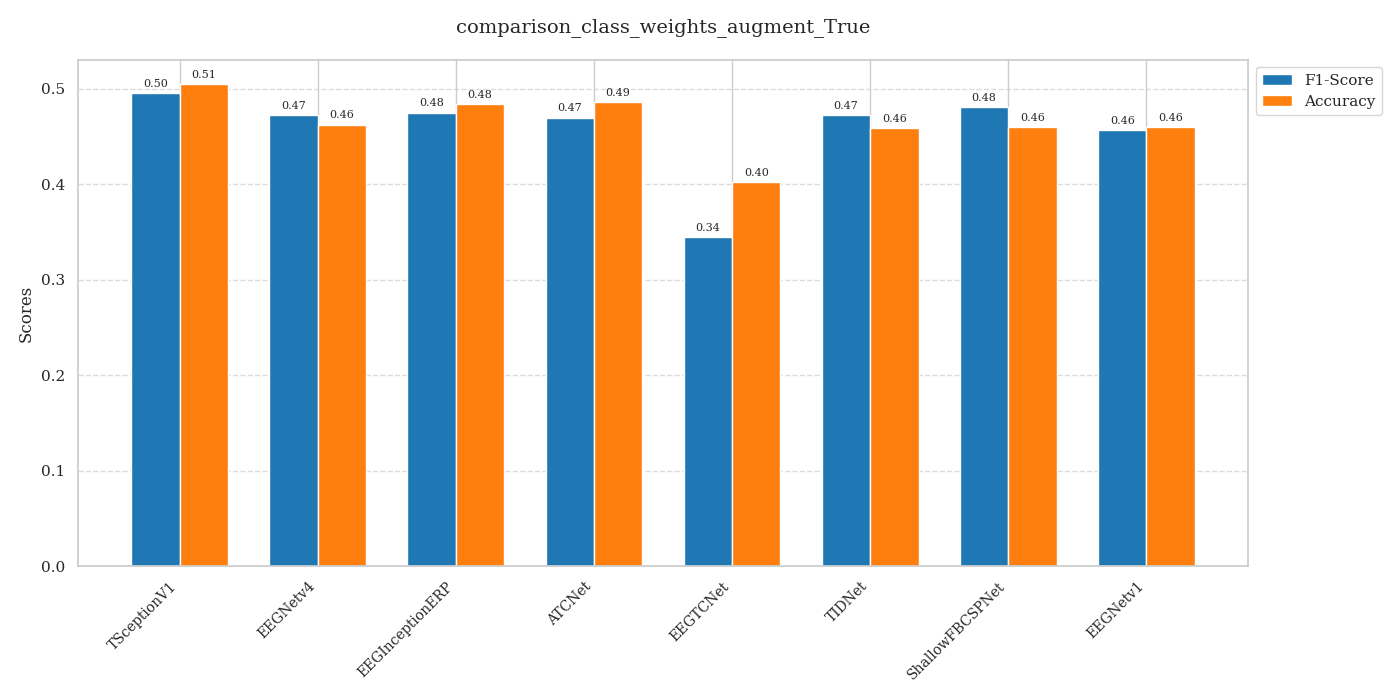
\includegraphics[width=1\linewidth]{images/comparison_class_weights_augment_True.png}
    \caption{Performanța modelelor cu weight-uri de clase și augmentari.}
    \label{fig:performance_class_weights_augment_true}
\end{figure}

\begin{figure}
    \centering
    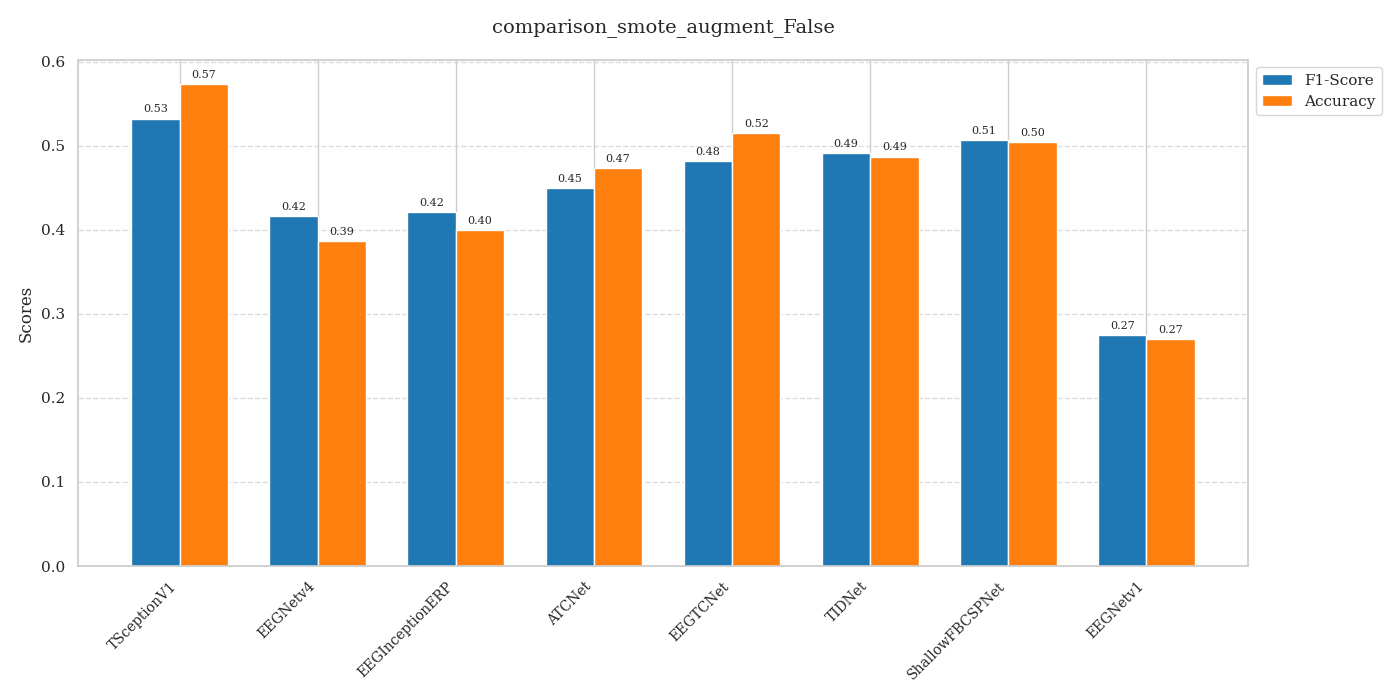
\includegraphics[width=1\linewidth]{images/comparison_smote_augment_False.png}
    \caption{Performanța modelelor folosind date sintetice, fără augmentări.}
    \label{fig:smote_augment_false}
\end{figure}

\begin{figure}
    \centering
    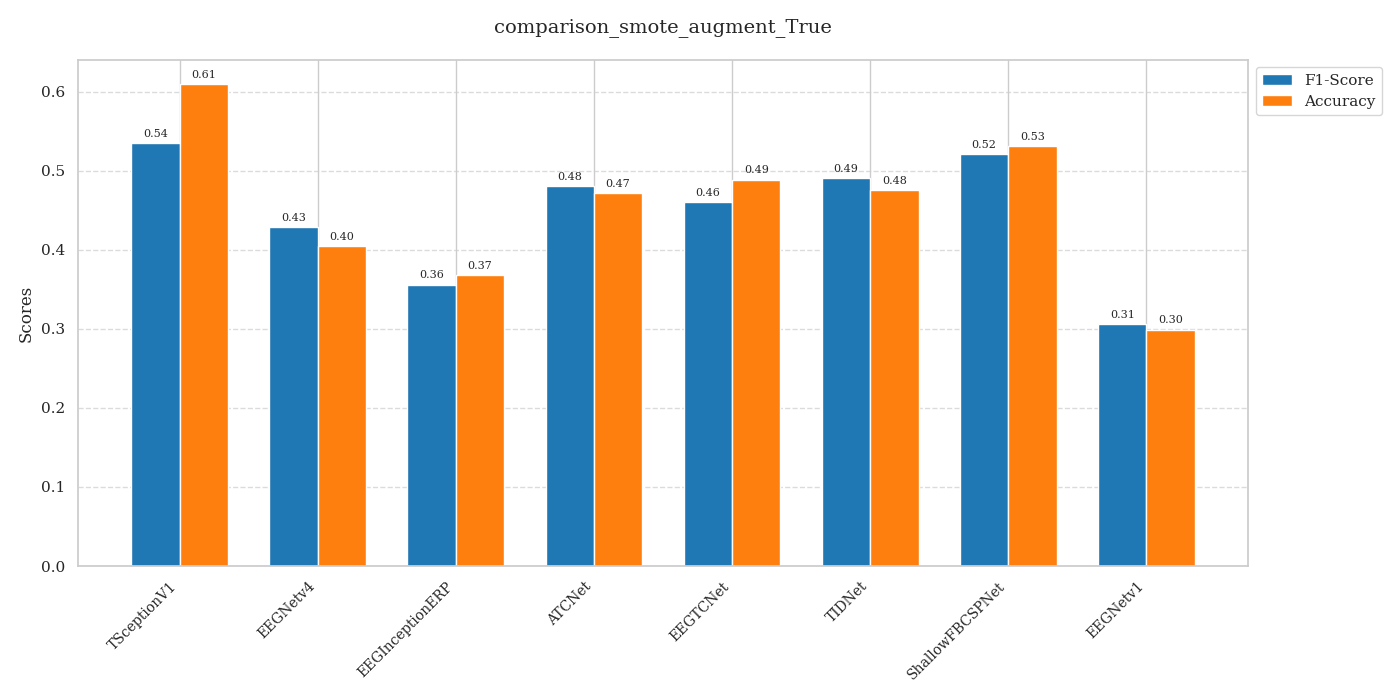
\includegraphics[width=1\linewidth]{comparison_smote_augment_True.png}
    \caption{Performanța modelelor, folosind date sintetice și augmentări.}
    \label{fig:smote_augment_true}
\end{figure}

\chapter{Cod sursă}

\begin{figure}[H]
\begin{lstlisting}[language=Python]
classifier = braindecode.classifier.EEGClassifier(
    model,
    criterion=torch.nn.CrossEntropyLoss,
    criterion__weight=torch.tensor(class_weights, dtype=torch.float32) if imbalance_mode=='class_weights' else None,
    train_split=predefined_split(torch.utils.data.TensorDataset(torch.tensor(X_valid).float(), torch.tensor(y_valid).long())),
    device='cuda',
    max_epochs=1000,
    callbacks=[skorch.callbacks.EarlyStopping(patience=20, load_best=True), skorch.callbacks.Checkpoint(), skorch.callbacks.LRScheduler()],
)
\end{lstlisting}
\caption{Apelarea wrapper-ului din braindecode.}
\label{fig:wrapper_braindecode}
\end{figure}

\begin{figure}[H]
\begin{lstlisting}[language=Python]
@ray.remote
def create_worker(participant, options):
    return EEGSubjectPipeline(participant, participant.replace("raw.csv", "quizz.xlsx"), 'dsi-24.elc', options)

workers = []
for participant in participants:
    workers.append(create_worker.remote(participant, options))

all_pipelines = ray.get(workers)

ray.shutdown()
\end{lstlisting}
\caption{Paralelizare utilizând Ray.}
\label{fig:paralelizare_ray}
\end{figure}


%\begin{figure}[h]
%    \centering
%    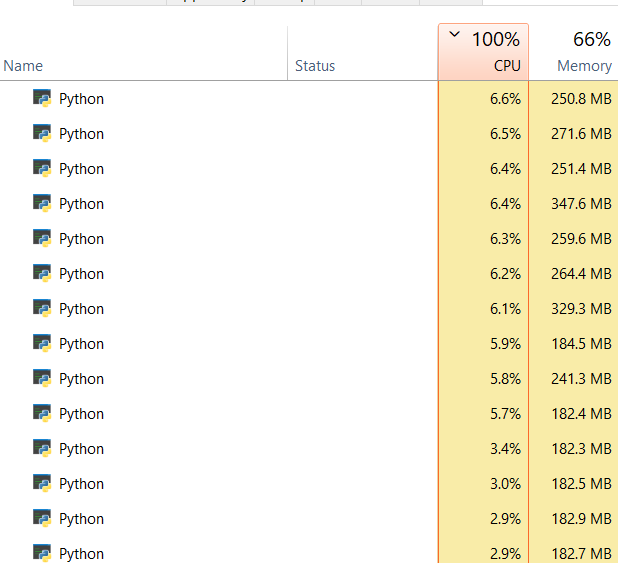
\includegraphics[width=0.7\linewidth]{task_manager.png}
%    \caption{Load-ul pe calculator}
%    \label{fig:load_calculator}
%\end{figure}

\begin{figure}
    \centering
    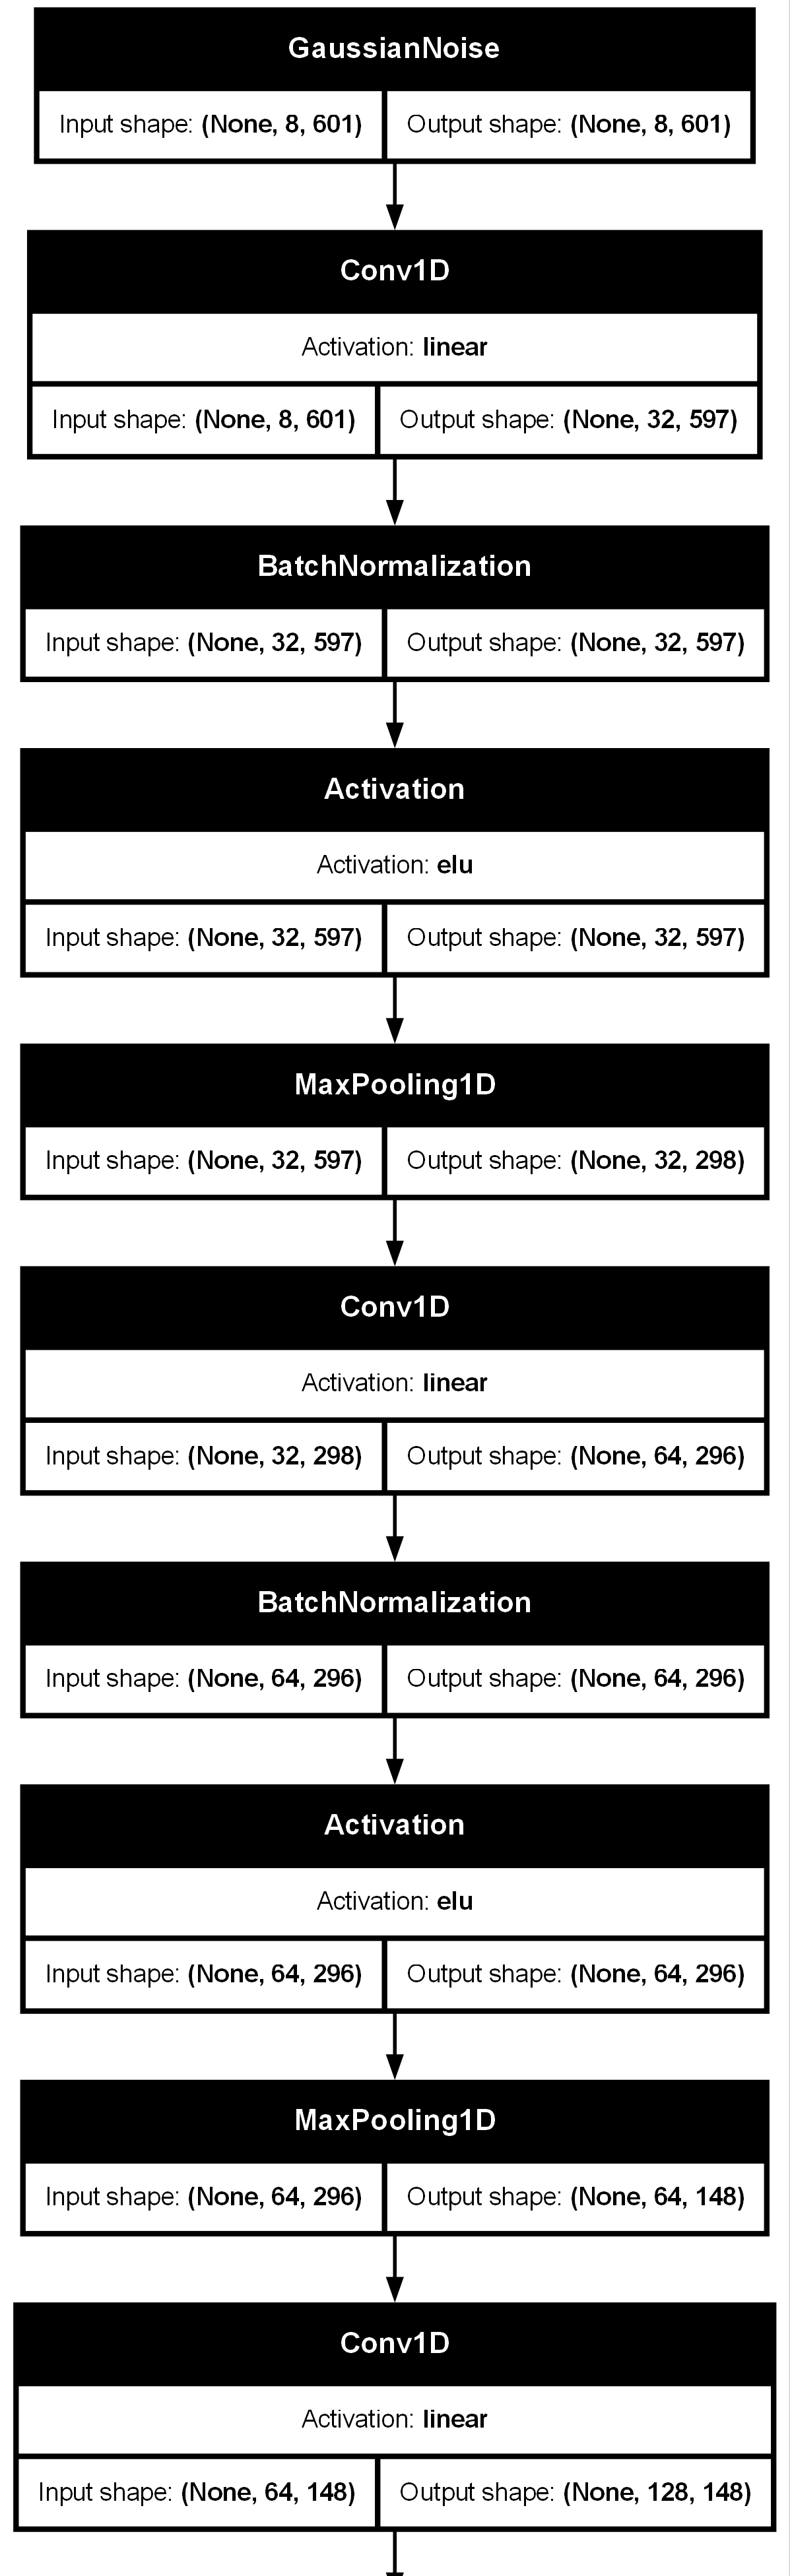
\includegraphics[width=0.4\linewidth]{model_part1.png}
    \caption{Model personal, partea 1.}
    \label{fig:model_part1}
\end{figure}

\begin{figure}
    \centering
    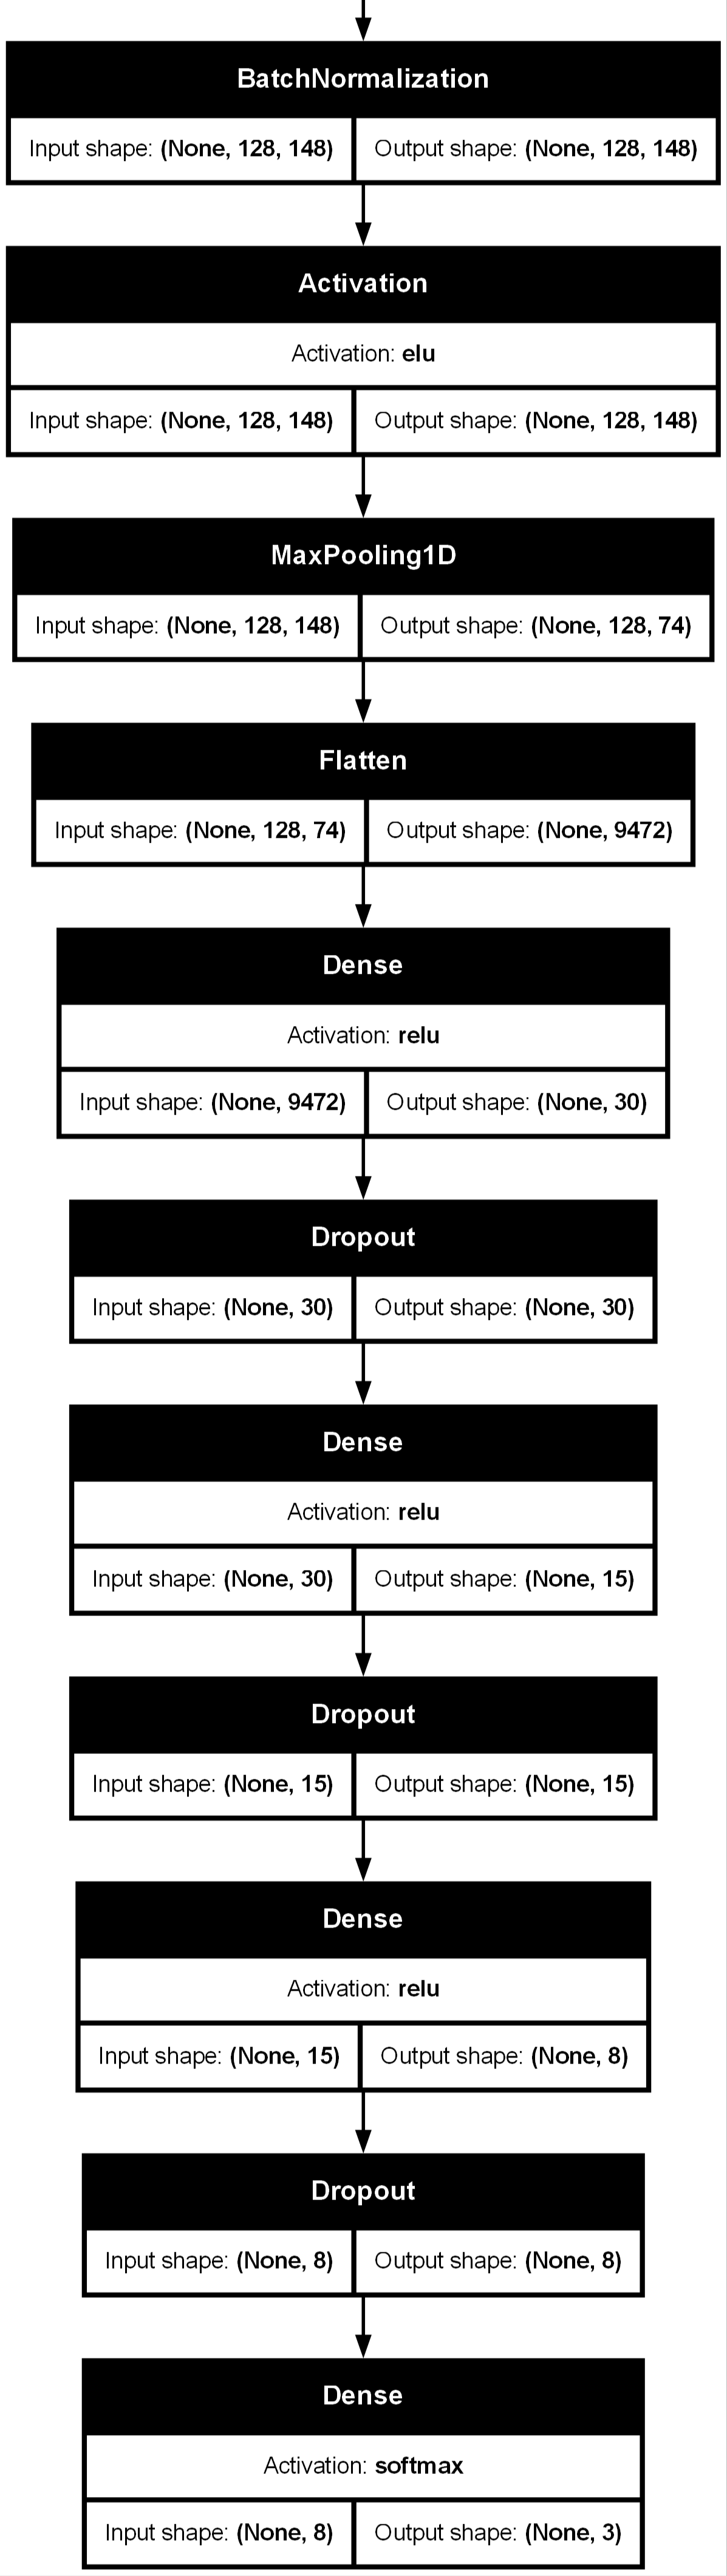
\includegraphics[width=0.4\linewidth]{model_part2.png}
    \caption{Model personal, partea 2.}
    \label{fig:model_part2}
\end{figure}

\begin{figure}
\begin{lstlisting}[language=Python]
def objective(trial):
    options = EEGpipelineOptions()

    options.interpolate_bad = trial.suggest_categorical('interpolate_bad', [False, True])
    options.apply_minmax_scaling_raw = trial.suggest_categorical('apply_minmax_scaling_raw', [False, True])
    options.apply_eog_regression = trial.suggest_categorical('apply_eog_regression', [False, True])
    options.apply_normalisation_raw = trial.suggest_categorical('apply_normalisation_raw', [False, True])
    options.apply_eeg_reference = trial.suggest_categorical('apply_eeg_reference', [False, True])

    options.apply_filters_raw = trial.suggest_categorical('apply_filters_raw', [False, True])
    options.apply_auto_ica_raw = False

    options.apply_manual_ica = False
    options.ica_components_raw = 20
    options.ica_threshold_raw = 2.5
    options.apply_autoreject = trial.suggest_categorical('apply_autoreject', [False, True])
    options.l_freq_raw = 4
    options.h_freq_raw = 40
    options.t_min = -0.2
    options.t_max = 1.8
    options.apply_xdawn_denoising = False
    options.apply_epoch_baseline = True

@ray.remote
def create_worker(participant, options):
    return EEGsubjectPipeline(participant, participant.replace("raw.csv", "quizz.xlsx"), "dsi-24.elc", options)

workers = []
for participant in participants:
    workers.append(create_worker_remote(participant, options))
all_pipelines = ray.get(workers)

ray.shutdown()

return get_model_metrics(braindecode.models.EEGNetv4(n_channels=n_chans, n_outputs=3, sfreq=300, n_times=601), all_pipelines)[1]

def callback(study, trial):
    if study.best_trial == trial:
        filehandler = open("output/braindecode_models/best_study.obj", "wb")
        pkl.dump(study, filehandler)
        filehandler.close()

study = optuna.create_study(direction="maximize")
study.optimize(objective, n_trials = 64, callbacks=[callback])
\end{lstlisting}
\caption{Căutarea hiperparametrilor folosind optuna.}
\label{fig:optuna_search}
\end{figure}

\begin{figure}
\begin{lstlisting}[language=Python]
def preprocess(self, apply_normalization = True, apply_minmax_scaling=True,
               apply_filters = True, apply_ica = True, apply_eog_regression = True,
               apply_manual_ica=True, apply_eeg_reference = True):
    if self.__isPreprocessed == True:
        return self
    self.__isPreprocessed = True
    if apply_eeg_reference:
        self.__apply_eeg_reference()
    if apply_filters:
        self.__filter_raw()
    if apply_eog_regression:
        self.__eog_regression()
    if apply_ica:
        self.__apply_auto_ica()
    if apply_manual_ica:
        self.__apply_ica()
    if apply_normalization:
        self.__normalize_raw()
    if apply_minmax_scaling:
        self.__minmax_scaling_raw()
    return self
\end{lstlisting}
\caption{Parametrizarea preprocesării semnalului.}
\label{fig:parametrizare}
\end{figure}

\begin{figure}
\begin{lstlisting}[language=Python]
if augment:
    X_train_jittered = add_temporal_jitter(X_train, jitter_range_ms=20, sampling_rate=300)
    X_train = np.concatenate([X_train, X_train_jittered], axis=0)
    y_train = np.concatenate([y_train, y_train], axis=0)

    X_train = torch.Tensor(X_train)
    y_train = torch.Tensor(y_train)
    X_train_noised, y_noised = braindecode.augmentation.GaussianNoise(probability=0.5) \
        .operation(X_train, y_train, std=0.1)
    X_train = X_train.detach().cpu().numpy()
    y_train = y_train.detach().cpu().numpy()

    X_train_noised = X_train_noised.detach().cpu().numpy()
    y_noised = y_noised.detach().cpu().numpy()
    X_train = np.concatenate([X_train, X_train_noised], axis=0)
    y_train = np.concatenate([y_train, y_noised], axis=0)

    X_train = torch.Tensor(X_train)
    y_train = torch.Tensor(y_train)
    X_train_noised, y_noised = braindecode.augmentation.SmoothTimeMask(probability=0.5) \
        .operation(X_train, y_train, mask_start_per_sample=torch.randint(low=0, high=400, size=(X_train.shape[0],)), 
                   mask_len_samples=40)
    X_train = X_train.detach().cpu().numpy()
    y_train = y_train.detach().cpu().numpy()

    X_train_noised = X_train_noised.detach().cpu().numpy()
    y_noised = y_noised.detach().cpu().numpy()
    X_train = np.concatenate([X_train, X_train_noised], axis=0)
    y_train = np.concatenate([y_train, y_noised], axis=0)
\end{lstlisting}
\caption{Codul folosit pentru agumentarea datelor.}
\label{fig:augmentari}
\end{figure}

\begin{figure}
\begin{lstlisting}[language=Python]
import pygad

all_features = ["mean", "variance", "std", "ptp_amp", "skewness", "kurtosis", "rms", "quantile", "hurst_exp",
                "app_entropy", "samp_entropy", "decorr_time", "pow_freq_bands", "hjorth_mobility_spect", "hjorth_complexity_spect",
                "hjorth_mobility", "hjorth_complexity", "higuchi_fd", "katz_fd", "zero_crossings", "line_length", "spect_slope",
                "spect_entropy", "svd_entropy", "svd_fisher_info", "energy_freq_bands", "spect_edge_freq", "wavelet_coef_energy",
                "teager_kaiser_energy"]

desired_output1 = 1
desired_output2 = 1

def fitness_func(ga_instance, solution, solution_idx):
    model = create_feature_pipeline(sklearn.neighbors.KNeighborsClassifier(), [x[0] for x in zip(all_features, solution) if x[1] > 0])
    output1, output2, _ = get_model_metrics(model, all_pipelines)
    return [output1, output2]

num_generations = 10
num_parents_mating = 10

sol_per_pop = 20
num_genes = len(all_features)

ga_instance = pygad.GA(num_generations=num_generations,
                       num_parents_mating = num_parents_mating,
                       sol_per_pop = sol_per_pop,
                       num_genes = num_genes,
                       fitness_func=fitness_func,
                       parent_selection_type='nsga2',
                       parallel_processing=('process', 8),
                       save_best_solutions=True,
                       save_solutions=True
                       )

ga_instance.run()
\end{lstlisting}
\caption{Configurația codului folosit pentru algoritmul genetic.}
\label{fig:pygad_configuration}
\end{figure}

\begin{figure}
\begin{lstlisting}[language=Python]
def create_pipeline(model):
    class Normalizer(sklearn.base.BaseEstimator, sklearn.base.TransformerMixin):
        def fit(self, X, y=None):
            self.mean = X.mean()
            self.std = X.std()
            return self

        def transform(self, X):
            return (X - self.mean) / self.std

    class FlattenTransformer(sklearn.base.BaseEstimator, sklearn.base.TransformerMixin):
        def fit(self, X, y=None):
            return self

        def transform(self, X):
            return X.reshape(X.shape[0], -1)

    steps = [("flatten", FlattenTransformer()), ("normalize", Normalizer()), ("scaler", sklearn.preprocessing.StandardScaler()), ("model", model)]
    pipe = Pipeline(steps)
    return pipe
\end{lstlisting}
\caption{Pipeline folosit pentru a normaliza și aplatiza datele trimise modelelor clasice.}
\label{fig:pipeline_modele_clasice}
\end{figure}

\end{document}